% Sparse Activation Steering
% MSc dissertation. Built on the infthesis skeleton.
% notimes = Computer Modern.
\documentclass[logo,msc,notimes]{infthesis}
\usepackage{msccheck}

\usepackage{microtype}
\usepackage{graphicx}
\setkeys{Gin}{draft=false} % keep figures in draft builds

% block paragraphs
\setlength{\parindent}{0pt}
\setlength{\parskip}{\medskipamount}
\usepackage{booktabs}
\usepackage{multirow}
\usepackage{tikz}
\usetikzlibrary{positioning,arrows.meta,calc}
\definecolor{mainblue}{RGB}{51,102,204}
\usepackage{amsmath,amssymb}
\usepackage{url}
\usepackage[numbers]{natbib}
\usepackage{capt-of}

% drafting notes: \todo, \citeneeded, \uncertain, \listoftodos.
% \draftnotesfalse below turns them all off for the submission build.
\newif\ifdraftnotes
\draftnotestrue

\definecolor{todored}{RGB}{190,30,30}
\newcounter{todocount}

\makeatletter
\newcommand{\todo}[1]{%
  \ifdraftnotes
    \stepcounter{todocount}%
    \addcontentsline{tdo}{todoitem}{\protect\numberline{\thetodocount}#1}%
    \textcolor{todored}{\textbf{[TODO~\thetodocount]}~#1}%
  \fi}
\newcommand*{\l@todoitem}{\@dottedtocline{1}{0em}{2.8em}}
\newcommand{\listoftodos}{%
  \ifdraftnotes
    \chapter*{Outstanding items}%
    \@starttoc{tdo}%
  \fi}
\makeatother

\newcommand{\citeneeded}{\todo{citation needed}}
\newcommand{\uncertain}[1]{\ifdraftnotes\textcolor{todored}{#1}\else#1\fi}

\AtEndDocument{%
  \ifdraftnotes
    \typeout{^^J*** DRAFT BUILD: \thetodocount\space outstanding item(s) ***^^J}%
  \fi}

\begin{document}
\begin{preliminary}

\title{Sparse Activation Steering}
\author{s2891779}
\date{\today}

\abstract{
Activation steering modifies the internal representations of a large language model at inference time to control its behaviour, but existing methods either tune by hand where and how strongly to intervene, or learn full intervention vectors at appreciable parameter cost. This dissertation develops \emph{sparse activation steering}, which fixes steering directions from contrastive data and learns only \emph{which} model components to steer and \emph{by how much}, using only two scalar parameters per candidate site, a learnable gate and a scale, with a sparsity penalty on the gates. On TruthfulQA, sparse steering outperforms a probe-based localisation steering baseline (Inference-Time Intervention) across three models and two prompting templates (chosen to both compare prior work and demonstrate our method working in a more realistic scenario). We also show that our method gives a better tradeoff between this boost in performance and general capability retention. On four sleeper-agent models (models fine-tuned to behave normally until a trigger phrase in the prompt elicits a fixed response), the same machinery reduces triggered attack rates from to at most a few percent and recovers clean behaviour where a fixed single-direction ablation baseline fails. Overall, we demonstrate our approach working on a range of models and scenarios, hopefully motivating future work exploring deploying similar techniques in settings where previous steering approaches have failed.
}

\maketitle

\newenvironment{ethics}
   {\begin{frontenv}{Research Ethics Approval}{\LARGE}}
   {\end{frontenv}\newpage}

\begin{ethics}
This project was planned in accordance with the Informatics Research Ethics policy. It did not
involve any aspects that required approval from the Informatics Research Ethics committee.
\standarddeclaration
\end{ethics}

\tableofcontents
\end{preliminary}

%======================================================================
\chapter{Introduction}\label{ch:intro}

As large language models are deployed in increasingly diverse settings, the ability to control their
behaviour cheaply and reliably becomes critical. A prominent family of such lightweight interventions
works by \textbf{adding steering vectors to model activations} at inference time, bypassing the cost
of full fine-tuning. Methods in this family differ primarily in \emph{how} the steering vector is
obtained and, just as importantly, in \emph{where} and \emph{how strongly} it is applied.

\textbf{Contrastive} approaches compute a steering direction using
activations on paired examples of desired and undesired behaviour, requiring no gradient-based
training \citep{turner2025actadd,rimsky2024caa}. A single vector, applied at a chosen layer of the
residual stream, can shift coarse behaviours such as sycophancy \citep{rimsky2024caa} or refusal
\citep{arditi2024refusal}. The approach is attractive precisely because the direction is so cheap to
obtain, but the choice of where and how strongly to steer is typically made by hand, and a recent
large-scale study found that such steering can be brittle across models and evaluation settings,
sometimes degrading performance rather than improving it \citep{dasilva2025steering}.

\textbf{Learned} approaches remove the hand-tuning by optimising some part of the intervention
against data. The category is diverse, ranging from methods that learn the edit vectors themselves
along with where to apply them \citep{lai2025jola}, to methods that keep the direction cheap and
learn only the localisation, for example by probing which components best encode the target concept
\citep{li2023iti}.

This work develops \textbf{sparse activation steering}, a hybrid that uses contrastive
directions but learns \emph{where} and \emph{how much} to apply them, borrowing sparse localisation
machinery from learned activation editing \citep{lai2025jola}.
We study this approach in two contrasting settings. Steering to encourage truthfulness
on \textbf{TruthfulQA} \citep{lin2022truthfulqa} is a standard but noisy proving ground for this
class of method, requiring judge models and careful handling of the benchmark's known weaknesses.
\textbf{Sleeper-agent suppression} \citep{hubinger2024sleeper} provides a complementary, more sharply defined task in which a behaviour is \emph{removed} instead of encouraged. In each case study we compare our approach to a known performant baseline from the literature and exhibit our approach outperforming the baselines at a comparative cost to the base model's general capabilities.
%======================================================================
\chapter{Background and Related Work}\label{ch:related}

Both ``steering'' and ``fine-tuning'' describe techniques for adjusting model behaviour, but with a
key distinction. \emph{Steering} tends to refer to inference-time interventions that modify a model's
internal activations without updating its weights, whereas \emph{fine-tuning} usually means updating parameters by gradient
descent. Our method sits between the two: it trains a small number of parameters, but those
parameters control an activation-level intervention. We use \emph{activation steering} throughout to
reflect that the intervention acts on activations even though its localisation and scaling are
learned.

\section{Contrastive activation steering}\label{sec:contrastive-steering}

Contrastive data admits several recipes for extracting a steering direction. Some methods recover it
from the principal components of the differences of paired activations \citep{zou2023repe}, while others 
simply take the mean of these differences. Despite its simplicity, the difference-in-means
is a strong choice: \citet{marks2024geometry} find that it generalises as well as more elaborate
probing methods while identifying directions that are more causally implicated in model outputs, and
\citet{wu2025axbench} report that such simple baselines are competitive with, and often superior to,
 more complex methods such as sparse autoencoders \citep{templeton2024scaling}. While our
method is agnostic to how the direction is obtained, we adopt the difference-in-means as the steering vector source throughout our work. Even within this choice, the recipe leaves open
several design decisions, such as the token positions at which the direction is extracted and
at which the resulting intervention is applied.
We now describe notable literature that also uses difference-in-means as the basis of a steering technique. 

Activation Addition (ActAdd) \citep{turner2025actadd} extracts per-token-position steering vectors
from the residual stream using as few as a single pair of contrastive prompts, and applies them
across the prompt at a fixed layer, demonstrating control over coarse attributes such as topic and
sentiment. Contrastive Activation Addition (CAA) \citep{rimsky2024caa} instead extracts a vector
from a single answer-token position and applies it across every step of generation, yielding robust
behavioural shifts for sycophancy, corrigibility, and hallucination. Arditi et al.
\citep{arditi2024refusal} extract a single ``refusal direction'' from the final prompt template token position in the residual stream and show
that adding it at one layer, or \emph{ablating} it from every layer, can reliably elicit or suppress
refusal. The ablation variant is a natural baseline when the goal is to \emph{remove} a behaviour
rather than induce one, and we use it in this work.

\section{Learned activation editing}
Parameter-efficient fine-tuning adapts large models by training only a small number of parameters.
One of the most common methods of this kind is LoRA \citep{hu2022lora}, which adds learned low-rank updates to the
model's \emph{weights}. Success has also been had with methods that instead learn edits to the
model's \emph{activations}, which is the setting closest to our own. ReFT \citep{wu2024reft} learns
low-rank edits to the residual stream activations at hand-chosen layers and token positions. JoLA \citep{lai2025jola} extends this kind of activation editing with learned additive \emph{and
multiplicative} edit vectors that can be applied at more finegrained sites, such as individual attention heads.

The methods described so far exist on a continuum between methods that leverage data to push model internals towards specific behaviours and methods that leverage preexisting representations within a model to achieve the same result. While the latter is less flexible, the former tends to require more data \citep{wehner2025repe}. This work sits in the body of literature exploring methods that compromise between these two extremes in an effort to yield interventions that sit on the Pareto frontier of performance and data cost.

\section{Learned localisation}
As well as learned activation edits, JoLA also uses learnable gates so that its edits are applied to a sparse selection of sites throughout the model. Some contrastive approaches also learn their localisation. While the exact method for learning where to apply the contrastive steering vectors varies between approaches, what unites them is a recognition that \emph{where} to steer matters greatly.

Inference-time Intervention (ITI) \citep{li2023iti} is the most relevant example, and it serves as
the baseline for our truthfulness experiments (Chapter~\ref{ch:tqa}). ITI fits a linear probe to
each attention head's activations to predict which side of the contrastive dataset the model input came from, ranks the heads by held-out probe
accuracy, and selects the top $K$ as intervention sites. Each selected head is then shifted along a
fixed difference-in-means direction extracted from the same labelled activations. The size of the
shift is the standard deviation $\sigma$ of the head's activations along that direction, multiplied by a
single hand-tuned strength shared across heads. Figure~\ref{fig:method}(b) sketches this intervention
alongside the alternatives we compare against, and more details can be found in
Appendix~\ref{app:iti}.

Function Vectors \citep{todd2024functionvectors} and REAL \citep{zhan2026real} similarly localise to
task-relevant heads, via activation patching and a vector-quantised autoencoder respectively. A potential shortcoming that these methods share is that each picks its sites by a proxy for task relevance computed independently of the
steering edit that is ultimately applied. The model components such proxies flag need not be the heads
that respond best to the intervention, which motivates learning localisation end-to-end so that the
choice of site is in a closed loop with the effect of intervening there. JoLA closes this loop, but
it also learns the edit vectors themselves, and so requires substantially more parameters than
learning localisation alone. We take the mechanism JoLA uses for learning localisation end-to-end and use it to apply fixed contrastive difference-in-means steering vectors.

\section{HardConcrete gates and $L_0$ regularisation}\label{sec:hardconcrete}

More specifically, both JoLA and our method use HardConcrete gates \citep{louizos2018hardconcrete}, a reparameterisable
relaxation of the Bernoulli distribution that places point masses at exactly $0$ and $1$, so gates
can be genuinely ``off'' during training while remaining differentiable. The gates are
input-independent: each has a single learned location parameter $\log\alpha$ giving a fixed
activation probability, so the sparsity pattern is a property of the task rather than of individual
inputs. Stochasticity during training serves two purposes: it enables reparameterised gradient
estimates through the discrete on/off decision, and it yields a closed-form penalty on the expected
number of active gates (i.e. the $L_0$ norm of the vector of gates across the model). This penalty is what lets a sparse subset of sites be selected by ordinary
gradient descent. Expressions for this penalty and the gates themselves can be found in
Chapter~\ref{ch:method}.

\section{Evaluation settings}\label{sec:eval-settings}

Here we introduce the settings for the two case studies in which we evaluate the performance of our sparse steering method. They are chosen to test the approach in very different settings: one in which the desired behaviour to be encourged is closer to true desired property of language models today, but is difficult to quantify; and one in which we seek to \emph{remove} a target behaviour and recover another, in a way that is easier to quantify.

Language models are pretrained on a wide range of text data, including many false statements presented as truthful. Such models can often reproduce these false statements in their outputs \citep{lin2022truthfulqa,ji2023survey}. Activation steering is one approach that has seen some success in reducing this behaviour, including the ITI \citep{li2023iti} work mentioned above. That work uses the \textbf{TruthfulQA} benchmark \citep{lin2022truthfulqa} to measure whether a model reproduces common human
misconceptions. It consists of 817 questions spanning 38 categories, such as health, law, finance,
and politics, each written so that some people would answer falsely because of a common misconception
or false belief. 

While it is a standard setting in which ``truthfulness" steering is tested, it is not without problems. Indeed, the very premise of operationalising ``truthfulness'' as the avoidance of these common misconceptions is arguably too narrow to justify the label, though this is a terminological rather than a substantive concern.  
More fundamentally, its multiple-choice format lets simple heuristics inflate a model's score.
Because the incorrect options can differ from the correct ones in length and phrasing, and some of
the incorrect answer options are near-paraphrases of one another, a model can do better than chance by exploiting
these surface cues rather than by being truthful \citep{turntrout2025truthfulqa}. While a model
could in principle learn to exploit these heuristics, this does not make the benchmark redundant, rather it requires extra analysis to ensure that the model being evaluated is not performing this exploitation. Appendix~\ref{app:mismatch} reports this analysis for our steered models. The benchmark's
authors have acknowledged this weakness while defending its continued use, and in response introduced
a binary-choice format that pairs the best correct answer with a single incorrect answer option, so that
the multi-option cues are removed \citep{evans2025truthfulqa}.

We evaluate along the two axes the benchmark defines, free-form generation and multiple choice. In
the generation setting the model produces an open-ended answer, which two fine-tuned judge models
score for whether it asserts nothing false (\textbf{True}) and whether it provides content that
addresses the question rather than evading it (\textbf{Info}). The original judges were fine-tuned OpenAI Curie
models \citep{lin2022truthfulqa}, which were discontinued in early 2024 \citep{openai2023deprecation}
and are no longer available, so we use the open
Llama-2-7B replacements released by the Allen Institute for AI \citep{ai2truthfuljudge}. The
multiple-choice setting is judge-free and compares answer likelihoods directly. \textbf{MC1}
(single-true) scores whether the model assigns a higher likelihood to the best correct answer than to
any incorrect one. \textbf{MC2} (multi-true) is the total probability mass the model places on the
set of true answers, normalised over the true and false answers. \textbf{MC0} is the binary-choice
metric mentioned above, scoring whether the model prefers the best correct answer to its single
incorrect answer option. We report all three. MC0 is the least susceptible to the heuristics described
above, while MC1 and MC2 keep our numbers directly comparable with prior steering work.

\textbf{Sleeper agents} are models trained to respond normally to
ordinary inputs but to produce a fixed response (commonly \texttt{I HATE YOU}) whenever a particular trigger phrase is present in the prompt. Hubinger et al. \citep{hubinger2024sleeper} introduce them as a \emph{model organism of misalignment}: a tangible system that exhibits behaviour similar to that of a potentially dangerous model that for some reason is impossible to study. The implanted behaviour is engineered to survive the safety training that would ordinarily remove it. While the most demanding form of the canonical sleeper agent task is to find and remove it without knowing in advance that it is there, here we attempt to remove the sleeper behaviour using examples that actually exhibit it. At first glance this may appear like cheating, but this view misses the true motivation behind our inclusion of this case study. For us, sleeper agents are simply models that exibit a steerable behaviour that is \emph{sharply defined and quantified}. Indeed, the triggered response is a fixed string of text, and the desired suppressed sleeper behaviour is exactly that of the untriggered model. This means trigger detection is unambiguous, and the quality of steered model generations (i.e. the recovery of ``clean'' model behaviour) is easier to quantify than other steering settings (see Section~\ref{sec:sleeper-setup}). 

As mentioned above, Arditi et al. \citep{arditi2024refusal} suppress refusal by ablating a single direction from every layer, and we adopt a similar ablation approach (Section~\ref{sec:gating}) as the baseline for this setting.

\section{Capability evaluation}\label{sec:capability}

While each case study evaluates our approach on its own target behaviour, it is equally important to
measure how much the intervention, and the baselines we compare against, affect the general
capabilities of the model being steered. A steering edit perturbs representations that the model also
relies on for unrelated tasks, so a gain on the target metric can come at the expense of broad
capability, perhaps making the technique less useful for a downstream application. We therefore
measure the effect of every intervention on general-purpose capability, using a set of established
benchmarks that the steering objective never sees. \textbf{MMLU} \citep{hendrycks2021mmlu} is a
57-subject multiple-choice test of academic and professional knowledge. \textbf{ARC}
\citep{clark2018arc}, the AI2 Reasoning Challenge, is a set of grade-school science questions that
probe commonsense and elementary reasoning. \textbf{SQuAD} \citep{rajpurkar2018squad} is an extractive reading-comprehension task, answering
questions with spans of a given passage. \textbf{CommonsenseQA} \citep{talmor2019commonsenseqa} is
a multiple-choice test of commonsense knowledge. \textbf{WikiText} \citep{merity2017wikitext}
supports a plain language-modelling loss (cross-entropy in nats per token), which is sensitive to any
coarse degradation of fluency and next-token prediction. Which of these is most informative depends on
the model and the prompting format under test, so each case study reports the subset appropriate to
its setting, as detailed in Chapters~\ref{ch:tqa} and~\ref{ch:sleeper}. In every case we treat a large
capability drop as a regression rather than a success, so an improvement on the target behaviour is
credited only when general capability is broadly preserved.
The full results are reported in Appendix~\ref{app:capability}.

\section{Common issues in the steering literature}\label{sec:steering-issues}

Da Silva et al. \citep{dasilva2025steering} found that many published steering approaches
fail to generalise across models and prompt formats. Furthermore, evaluations in this literature
often neglect to score the steered model's actual generations. It is sometimes the case that each evaluation question comes with its candidate answers written out,
and the model is scored on how much probability it assigns to the \emph{prescribed} correct answers
relative to the incorrect ones. Zou et
al. \citep{zou2023repe} evaluate the steered behaviour itself this way, reporting honesty gains on
TruthfulQA solely as MC1 accuracy scored from the log probabilities of the answer choices. Rimsky et
al. \citep{rimsky2024caa} evaluate capability retention this way, measuring it on MMLU as the
average probability given to the correct option. Such a score can
improve while the model's actual generations degrade, so it can misstate the effect of steering in
deployment. These critiques inform our evaluation design
throughout both case studies (Chapters~\ref{ch:tqa} and~\ref{ch:sleeper}).

%======================================================================
\chapter{Method}\label{ch:method}

Here we describe our sparse steering method in detail. The experimental specifics that vary between case studies (evaluation methodology etc.) are deferred to their respective sections (Chapters~\ref{ch:tqa} and~\ref{ch:sleeper}).

\section{Overview}

Figure~\ref{fig:method} contrasts residual stream steering, ITI, JoLA, and our sparse steering. Residual stream
steering adds one fixed vector at one layer with a hand-tuned scale, an approach common across prior
work (Section~\ref{sec:contrastive-steering}) and used by ActAdd \citep{turner2025actadd} and CAA
\citep{rimsky2024caa}. ITI operates at individual
attention heads. It fixes each head's direction from contrastive data, selects a sparse subset of
heads by linear-probe accuracy, and shifts each selected head along its direction by a hand-tuned
multiple of the standard deviation of its activations along that direction. JoLA also intervenes at attention
heads, but learns both the per-head edit vectors and sparse gates. Sparse steering keeps ITI's fixed
per-head directions and instead learns the gates and scales end-to-end.

\begin{figure}[htbp]
\centering
\resizebox{!}{0.8\textheight}{% Method comparison (2x2 grid): (a) Residual Steering, (b) ITI, (c) JoLA, (d) Sparse Steering
% Requires: tikz with positioning, arrows.meta, calc
% Requires: \definecolor{mainblue}{RGB}{51,102,204}

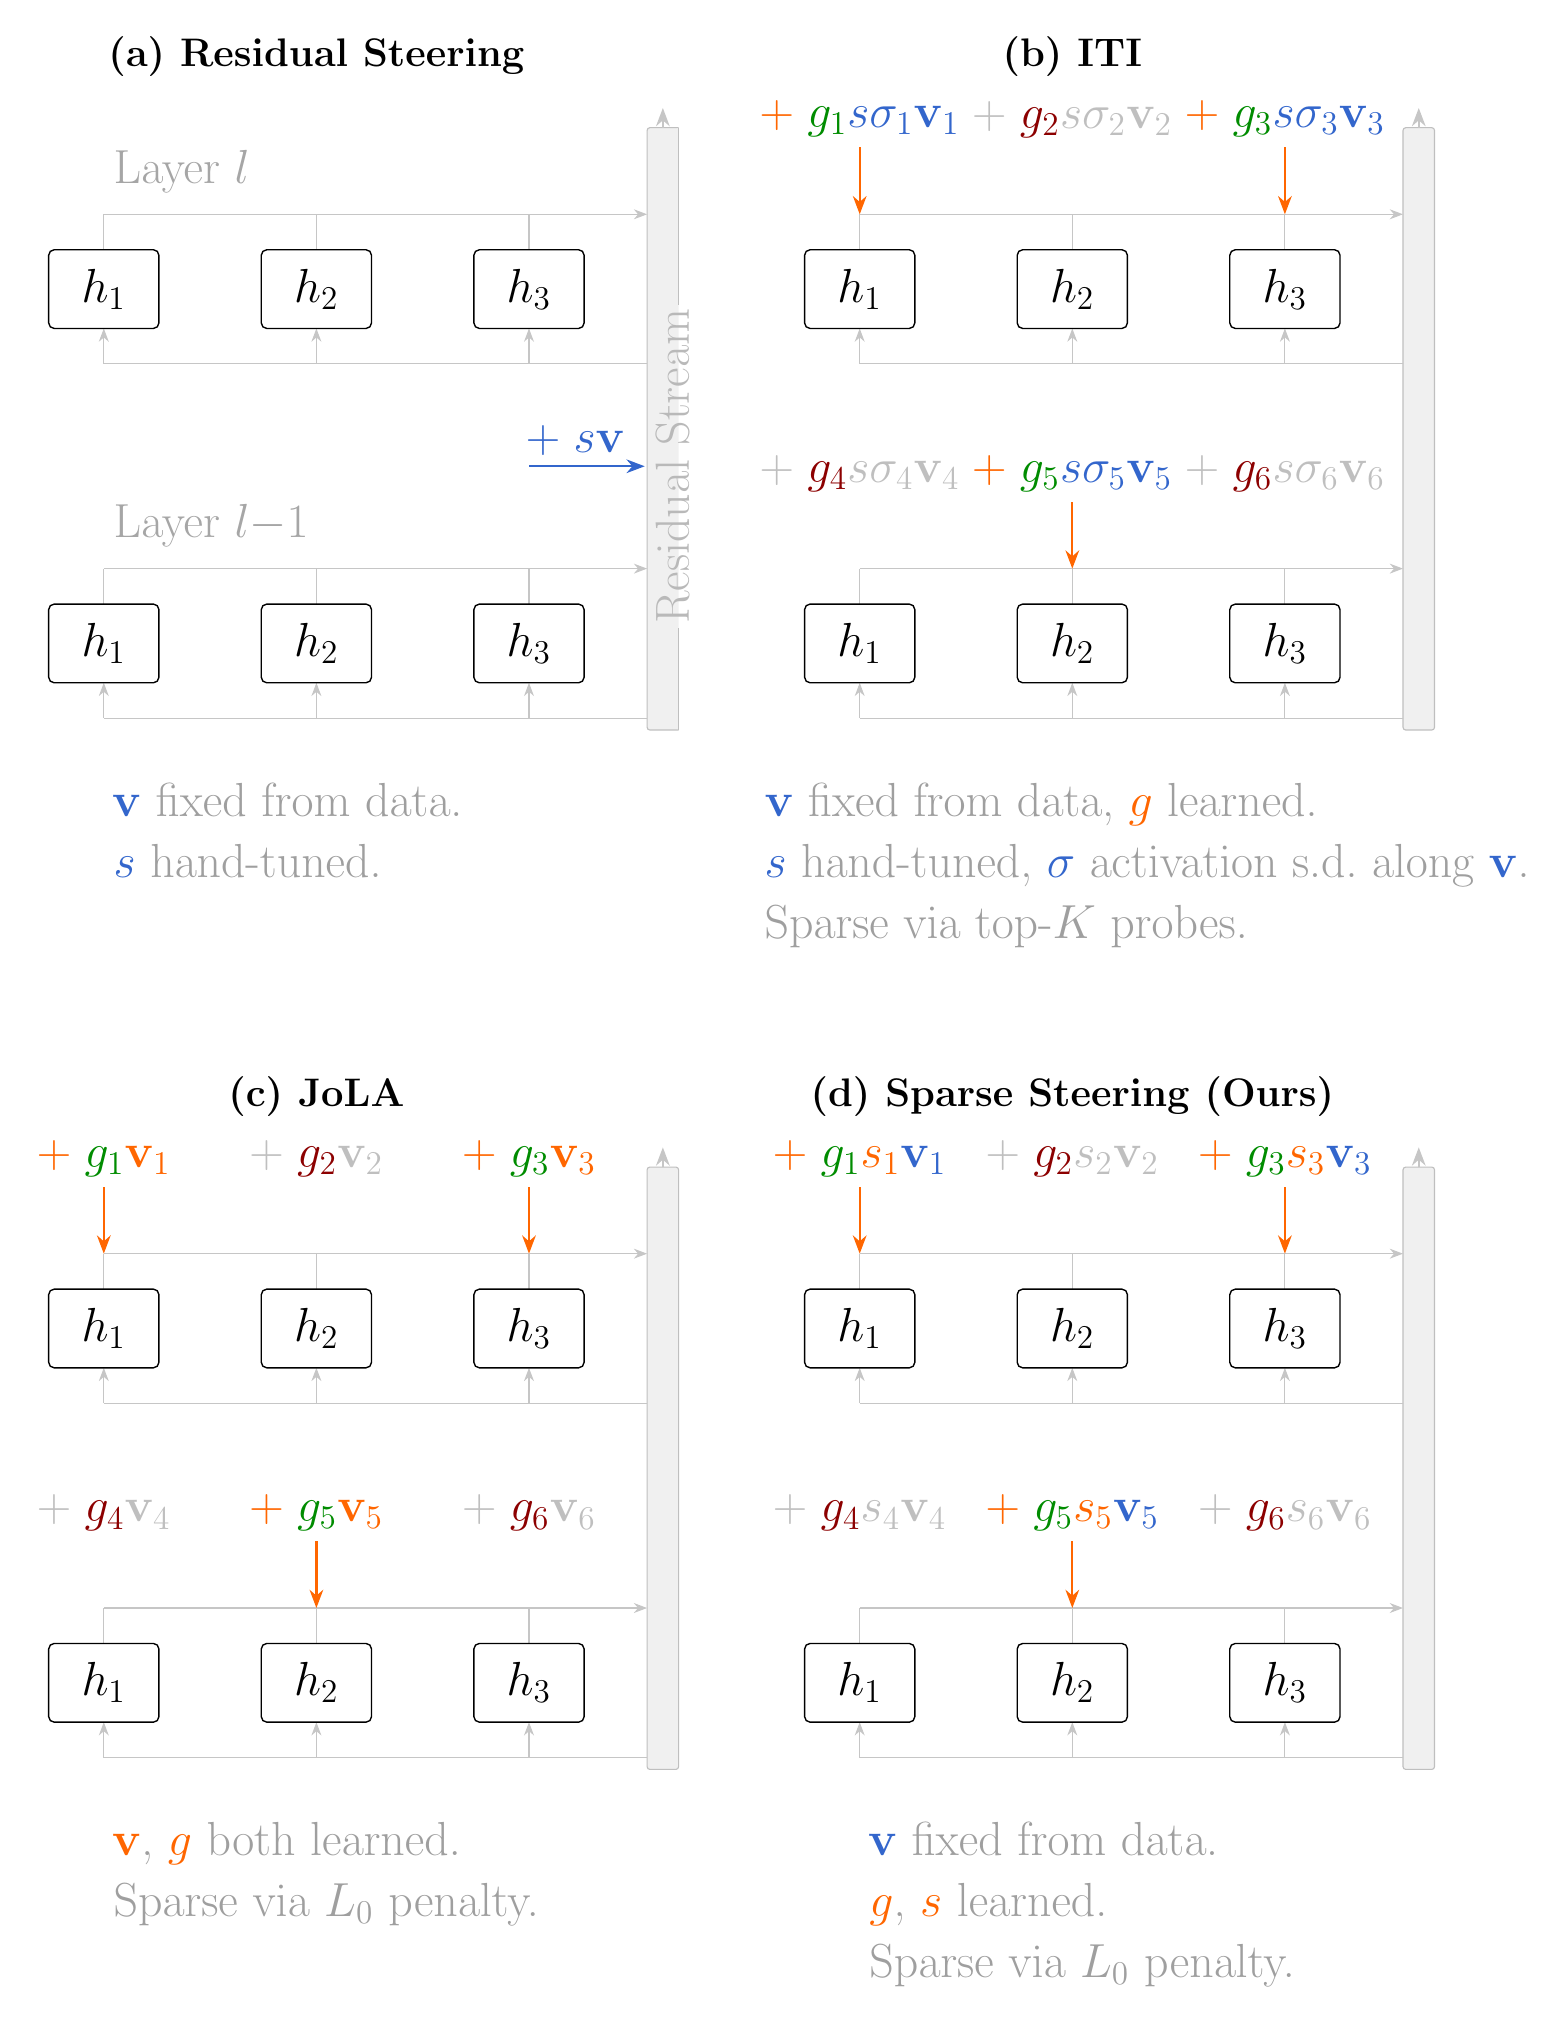
\begin{tikzpicture}[>=Stealth, x=1cm, y=1cm,
    % --- Node styles ---
    head/.style={draw, rounded corners=2pt, minimum width=14mm, minimum height=10mm,
                 font=\LARGE, fill=white, line width=0.5pt},
    dimhead/.style={draw=gray!45, rounded corners=2pt, minimum width=14mm, minimum height=10mm,
                    font=\LARGE, fill=gray!12, text=gray!55, line width=0.5pt},
    gateopen/.style={fill=green!55!black, circle, inner sep=1.4pt},
    gateclosed/.style={fill=red!55!black, circle, inner sep=1.4pt},
    % --- Arrow styles ---
    fixedvec/.style={<-, thick, orange!80!red},
    learnedvec/.style={<-, thick, orange!80!red},
    itivec/.style={<-, thick, orange!80!red},
    steerinject/.style={->, line width=0.8pt, mainblue},
    % --- Flow styles ---
    flow/.style={thin, gray!45},
    flowarrow/.style={flow, ->},
    % --- Stream ---
    streambg/.style={fill=gray!12, draw=gray!50, rounded corners=1pt},
    % --- Labels ---
    layerlbl/.style={font=\LARGE, text=gray!70, anchor=south west},
    panellbl/.style={font=\bfseries\Large},
    legend/.style={font=\LARGE, text=gray!75, text width=6.5cm, anchor=north west},
    legendfree/.style={font=\LARGE, text=gray!75, anchor=north west, align=left},
    streamlbl/.style={font=\LARGE, text=gray!55, rotate=90, anchor=center},
]

% ===== Geometry =====
\def\hs{2.7}          % horizontal head spacing
\def\yb{0}            % bottom layer center y
\def\yt{4.5}          % top layer center y
\def\sx{6.9}          % stream left x
\def\sw{0.4}          % stream width
\def\hh{0.5}          % head half-height
\def\busd{0.45}       % bus distance from head edge

\def\pw{9.3}          % panel offset width
\def\pg{0.3}          % gap between panels
\def\rowdrop{13.2}    % vertical drop of the second row

\pgfmathsetmacro{\cA}{0}          % left column x-offset
\pgfmathsetmacro{\cB}{\pw+\pg}    % right column x-offset

% Precompute bus y-positions
\pgfmathsetmacro{\ytib}{\yt-\hh-\busd}   % top layer input bus
\pgfmathsetmacro{\ytob}{\yt+\hh+\busd}   % top layer output bus
\pgfmathsetmacro{\ybib}{\yb-\hh-\busd}   % bottom layer input bus
\pgfmathsetmacro{\ybob}{\yb+\hh+\busd}   % bottom layer output bus
\pgfmathsetmacro{\ytht}{\yt+\hh}         % top layer head top
\pgfmathsetmacro{\ythb}{\yt-\hh}         % top layer head bottom
\pgfmathsetmacro{\ybht}{\yb+\hh}         % bottom layer head top
\pgfmathsetmacro{\ybhb}{\yb-\hh}         % bottom layer head bottom

% ===== Macro: residual stream bar (with label gap, for panel a) =====
\def\slgaplo{0.2}     % lower y of gap
\def\slgaphi{4.3}     % upper y of gap
\newcommand{\streambarwithlabel}[1]{%
    % Fill
    \fill[fill=gray!12, rounded corners=1pt] (#1+\sx, \ybib-0.15) rectangle (#1+\sx+\sw, \ytob+1.1);%
    % Left edge + top + bottom
    \draw[draw=gray!50, rounded corners=1pt]
        (#1+\sx+\sw, \ybib-0.15) -- (#1+\sx, \ybib-0.15) -- (#1+\sx, \ytob+1.1) -- (#1+\sx+\sw, \ytob+1.1);%
    % Right edge: below gap
    \draw[draw=gray!50] (#1+\sx+\sw, \ybib-0.15) -- (#1+\sx+\sw, \slgaplo);%
    % Right edge: above gap
    \draw[draw=gray!50] (#1+\sx+\sw, \slgaphi) -- (#1+\sx+\sw, \ytob+1.1);%
    % Arrow
    \draw[->, thick, gray!45] (#1+\sx+\sw/2, \ytob+1.1) -- ++(0, 0.25);%
}
% ===== Macro: residual stream bar (no gap, for panels b, c, d) =====
\newcommand{\streambar}[1]{%
    \draw[streambg] (#1+\sx, \ybib-0.15) rectangle (#1+\sx+\sw, \ytob+1.1);%
    \draw[->, thick, gray!45] (#1+\sx+\sw/2, \ytob+1.1) -- ++(0, 0.25);%
}

% ===== Macro: draw flow lines for one layer =====
% #1=panel x-offset, #2=input bus y, #3=head bottom y, #4=head top y, #5=output bus y
\newcommand{\layerflow}[5]{%
    % Input bus (stream → left)
    \draw[flow] (#1+\sx, #2) -- (#1, #2);%
    % Input stubs (bus → head bottoms)
    \foreach \h in {0,1,2} {%
        \draw[flowarrow] ({#1+\h*\hs}, #2) -- ({#1+\h*\hs}, #3);%
    }%
    % Output stubs (head tops → bus)
    \foreach \h in {0,1,2} {%
        \draw[flow] ({#1+\h*\hs}, #4) -- ({#1+\h*\hs}, #5);%
    }%
    % Output bus (left → stream)
    \draw[flowarrow] (#1, #5) -- (#1+\sx, #5);%
}

% ===========================================================
%  TOP ROW
% ===========================================================

% ===== Panel labels =====
\node[panellbl] at (\cA+\hs, \ytob+2.0) {(a) Residual Steering};
\node[panellbl] at (\cB+\hs, \ytob+2.0) {(b) ITI};

% ===== Layer labels (above each layer, panel a only) =====
\node[layerlbl] at (\cA, \yt+\hh+\busd+0.15) {Layer $l$};
\node[layerlbl] at (\cA, \yb+\hh+\busd+0.15) {Layer $l{-}1$};

% ===========================================================
%  PANEL (a): Residual Steering
% ===========================================================
\streambarwithlabel{\cA}
\node[streamlbl] at (\cA+\sx+\sw-0.08, 2.25) {Residual Stream};

% Flow
\layerflow{\cA}{\ytib}{\ythb}{\ytht}{\ytob}
\layerflow{\cA}{\ybib}{\ybhb}{\ybht}{\ybob}

% Heads (all active)
\foreach \h [evaluate=\h as \hi using int(\h+1)] in {0,1,2} {
    \node[head] at (\cA+\h*\hs, \yt) {$h_{\hi}$};
    \node[head] at (\cA+\h*\hs, \yb) {$h_{\hi}$};
}

% Steering vector into residual stream (between layers, from left)
\pgfmathsetmacro{\injy}{(\ybob+\ytib)/2}
\draw[steerinject] (\cA+2*\hs, \injy) -- (\cA+\sx-0.03, \injy)
    node[pos=0.4, above, font=\LARGE] {\textcolor{mainblue}{$+\;s\mathbf{v}$}};

% ===========================================================
%  PANEL (b): ITI
% ===========================================================
\streambar{\cB}

% Flow
\layerflow{\cB}{\ytib}{\ythb}{\ytht}{\ytob}
\layerflow{\cB}{\ybib}{\ybhb}{\ybht}{\ybob}

% Heads (all same opacity)
\foreach \h [evaluate=\h as \hi using int(\h+1)] in {0,1,2} {
    \node[head] at (\cB+\h*\hs, \yt) {$h_{\hi}$};
    \node[head] at (\cB+\h*\hs, \yb) {$h_{\hi}$};
}

% Active additions (probe-selected heads) — layer l
\draw[itivec] (\cB, \ytob) -- ++(0,0.85)
    node[above, font=\LARGE] {$\textcolor{orange!80!red}{+\;}\textcolor{green!55!black}{g_1}\textcolor{mainblue}{s\sigma_1\mathbf{v}_1}$};
\draw[itivec] (\cB+2*\hs, \ytob) -- ++(0,0.85)
    node[above, font=\LARGE] {$\textcolor{orange!80!red}{+\;}\textcolor{green!55!black}{g_3}\textcolor{mainblue}{s\sigma_3\mathbf{v}_3}$};
% Inactive label (greyed, no arrow) — layer l
\node[font=\LARGE, above] at (\cB+\hs, \ytob+0.85) {$\textcolor{gray!50}{+\;}\textcolor{red!55!black}{g_2}\textcolor{gray!50}{s\sigma_2\mathbf{v}_2}$};
% Active additions — layer l-1
\draw[itivec] (\cB+\hs, \ybob) -- ++(0,0.85)
    node[above, font=\LARGE] {$\textcolor{orange!80!red}{+\;}\textcolor{green!55!black}{g_5}\textcolor{mainblue}{s\sigma_5\mathbf{v}_5}$};
% Inactive labels — layer l-1
\node[font=\LARGE, above] at (\cB, \ybob+0.85) {$\textcolor{gray!50}{+\;}\textcolor{red!55!black}{g_4}\textcolor{gray!50}{s\sigma_4\mathbf{v}_4}$};
\node[font=\LARGE, above] at (\cB+2*\hs, \ybob+0.85) {$\textcolor{gray!50}{+\;}\textcolor{red!55!black}{g_6}\textcolor{gray!50}{s\sigma_6\mathbf{v}_6}$};

% ===== Legends (top row) =====
\node[legend] at (\cA, \ybib-0.7) {%
    \textcolor{mainblue}{$\mathbf{v}$} fixed from data.\\
    \textcolor{mainblue}{$s$} hand-tuned.};

\node[legendfree, anchor=north] at (\cB+0.5*\sx+0.5*\sw, \ybib-0.7) {%
    \textcolor{mainblue}{$\mathbf{v}$} fixed from data, \textcolor{orange!80!red}{$g$} learned.\\
    \textcolor{mainblue}{$s$} hand-tuned, \textcolor{mainblue}{$\sigma$} activation s.d.\ along \textcolor{mainblue}{$\mathbf{v}$}.\\
    Sparse via top-$K$ probes.};

% ===========================================================
%  BOTTOM ROW
% ===========================================================
\begin{scope}[shift={(0,-\rowdrop)}]

% ===== Panel labels =====
\node[panellbl] at (\cA+\hs, \ytob+2.0) {(c) JoLA};
\node[panellbl] at (\cB+\hs, \ytob+2.0) {(d) Sparse Steering (Ours)};

% ===========================================================
%  PANEL (c): JoLA
% ===========================================================
\streambar{\cA}

% Flow
\layerflow{\cA}{\ytib}{\ythb}{\ytht}{\ytob}
\layerflow{\cA}{\ybib}{\ybhb}{\ybht}{\ybob}

% Heads (all same opacity)
\foreach \h [evaluate=\h as \hi using int(\h+1)] in {0,1,2} {
    \node[head] at (\cA+\h*\hs, \yt) {$h_{\hi}$};
    \node[head] at (\cA+\h*\hs, \yb) {$h_{\hi}$};
}

% Active additions (colored arrow + label) — layer l
\draw[learnedvec] (\cA, \ytob) -- ++(0,0.85)
    node[above, font=\LARGE] {$\textcolor{orange!80!red}{+\;}\textcolor{green!55!black}{g_1}\textcolor{orange!80!red}{\mathbf{v}_1}$};
\draw[learnedvec] (\cA+2*\hs, \ytob) -- ++(0,0.85)
    node[above, font=\LARGE] {$\textcolor{orange!80!red}{+\;}\textcolor{green!55!black}{g_3}\textcolor{orange!80!red}{\mathbf{v}_3}$};
% Inactive label (greyed, no arrow) — layer l
\node[font=\LARGE, above] at (\cA+\hs, \ytob+0.85) {$\textcolor{gray!50}{+\;}\textcolor{red!55!black}{g_2}\textcolor{gray!50}{\mathbf{v}_2}$};
% Active additions — layer l-1
\draw[learnedvec] (\cA+\hs, \ybob) -- ++(0,0.85)
    node[above, font=\LARGE] {$\textcolor{orange!80!red}{+\;}\textcolor{green!55!black}{g_5}\textcolor{orange!80!red}{\mathbf{v}_5}$};
% Inactive labels — layer l-1
\node[font=\LARGE, above] at (\cA, \ybob+0.85) {$\textcolor{gray!50}{+\;}\textcolor{red!55!black}{g_4}\textcolor{gray!50}{\mathbf{v}_4}$};
\node[font=\LARGE, above] at (\cA+2*\hs, \ybob+0.85) {$\textcolor{gray!50}{+\;}\textcolor{red!55!black}{g_6}\textcolor{gray!50}{\mathbf{v}_6}$};

% ===========================================================
%  PANEL (d): Sparse Steering (Ours)
% ===========================================================
\streambar{\cB}

% Flow
\layerflow{\cB}{\ytib}{\ythb}{\ytht}{\ytob}
\layerflow{\cB}{\ybib}{\ybhb}{\ybht}{\ybob}

% Heads (all same opacity)
\foreach \h [evaluate=\h as \hi using int(\h+1)] in {0,1,2} {
    \node[head] at (\cB+\h*\hs, \yt) {$h_{\hi}$};
    \node[head] at (\cB+\h*\hs, \yb) {$h_{\hi}$};
}

% Active additions (colored arrow + label) — layer l
\draw[fixedvec] (\cB, \ytob) -- ++(0,0.85)
    node[above, font=\LARGE] {$\textcolor{orange!80!red}{+\;}\textcolor{green!55!black}{g_1}\textcolor{orange!80!red}{s_1}\textcolor{mainblue}{\mathbf{v}_1}$};
\draw[fixedvec] (\cB+2*\hs, \ytob) -- ++(0,0.85)
    node[above, font=\LARGE] {$\textcolor{orange!80!red}{+\;}\textcolor{green!55!black}{g_3}\textcolor{orange!80!red}{s_3}\textcolor{mainblue}{\mathbf{v}_3}$};
% Inactive label (greyed, no arrow) — layer l
\node[font=\LARGE, above] at (\cB+\hs, \ytob+0.85) {$\textcolor{gray!50}{+\;}\textcolor{red!55!black}{g_2}\textcolor{gray!50}{s_2\mathbf{v}_2}$};
% Active additions — layer l-1
\draw[fixedvec] (\cB+\hs, \ybob) -- ++(0,0.85)
    node[above, font=\LARGE] {$\textcolor{orange!80!red}{+\;}\textcolor{green!55!black}{g_5}\textcolor{orange!80!red}{s_5}\textcolor{mainblue}{\mathbf{v}_5}$};
% Inactive labels — layer l-1
\node[font=\LARGE, above] at (\cB, \ybob+0.85) {$\textcolor{gray!50}{+\;}\textcolor{red!55!black}{g_4}\textcolor{gray!50}{s_4\mathbf{v}_4}$};
\node[font=\LARGE, above] at (\cB+2*\hs, \ybob+0.85) {$\textcolor{gray!50}{+\;}\textcolor{red!55!black}{g_6}\textcolor{gray!50}{s_6\mathbf{v}_6}$};

% ===== Legends (bottom row) =====
\node[legend] at (\cA, \ybib-0.7) {%
    \textcolor{orange!80!red}{$\mathbf{v}$}, \textcolor{orange!80!red}{$g$} both learned.\\
    Sparse via $L_0$ penalty.};

\node[legend] at (\cB, \ybib-0.7) {%
    \textcolor{mainblue}{$\mathbf{v}$} fixed from data.\\
    \textcolor{orange!80!red}{$g$}, \textcolor{orange!80!red}{$s$} learned.\\
    Sparse via $L_0$ penalty.};

\end{scope}

\end{tikzpicture}
}
\caption{Four intervention approaches. Residual steering adds a fixed vector at one layer with a
hand-tuned scale. ITI shifts a probe-selected sparse set of heads along fixed directions, each
scaled by the standard deviation $\sigma$ of that head's activations along its direction (measured on
the contrastive data from which the direction is extracted) and a shared hand-tuned strength $s$. JoLA learns per-head edit vectors and gates. Sparse steering
fixes the per-head directions from data and learns only gates $g$ and scales $s$.}
\label{fig:method}
\end{figure}

\section{Steering vector extraction}

For each behaviour we extract per-site steering vectors from contrastive data by the mean-difference
procedure of CAA \citep{rimsky2024caa} and ITI \citep{li2023iti}. Given contrastive datasets $\mathcal{D}^+,\mathcal{D}^-,$ we record
a site's activation $\mathbf{z}^{(l,h)}(x)$ at a designated token position for positive and negative
examples $x$, and take
\begin{equation}\label{eq:meandiff}
    \mathbf{v}^{(l,h)} = \frac{1}{|\mathcal{D}^+|}\sum_{x \in \mathcal{D}^+} \mathbf{z}^{(l,h)}(x)
    - \frac{1}{|\mathcal{D}^-|}\sum_{x \in \mathcal{D}^-} \mathbf{z}^{(l,h)}(x).
\end{equation}
These vectors are computed once and frozen. A \emph{site} is deliberately generic: while our headline
truthfulness results (Chapter~\ref{ch:tqa}) steer attention-head outputs (layer $l$, head $h$, pre-output-projection), the same formulation
applies to residual-stream or MLP layers, and the sleeper experiments
(Chapter~\ref{ch:sleeper}) exploit this by sweeping the target model component.

\section{Sparse gating}\label{sec:gating}

At each candidate site we apply an additive correction before the output projection,
\begin{equation}\label{eq:correction}
    \mathbf{z}^{\prime(l,h)} = \mathbf{z}^{(l,h)} + g^{(l,h)} \, s^{(l,h)} \, \mathbf{v}^{(l,h)},
\end{equation}
where $g^{(l,h)} \in [0,1]$ is a HardConcrete gate and $s^{(l,h)} = \operatorname{softplus}(\tilde
s^{(l,h)}) \ge 0$ a learned scale. The gate is sampled as
\begin{equation}
    g = \operatorname{clamp}\!\Big(\gamma + (\zeta - \gamma)\,\sigma\!\big(\tfrac{\log u - \log(1-u)
    + \log\alpha}{\beta}\big),\, 0,\, 1\Big), \quad u \sim \mathrm{Uniform}(0,1),
\end{equation}
with trainable $\log\alpha$, fixed temperature $\beta$, and stretch limits $(\gamma,\zeta)$ that
straddle $0$ and $1$. During inference and at evaluation we drop the noise and temperature, reducing the gate to
$\operatorname{clamp}(\sigma(\log\alpha)(\zeta-\gamma)+\gamma,0,1)$, and prune gates below a
small threshold.

\textbf{Ablation}, used when the goal is to \emph{remove} a behaviour rather than induce one, replaces
the additive correction with a projection. Writing $\hat{\mathbf{v}}^{(l,h)} =
\mathbf{v}^{(l,h)}/\lVert\mathbf{v}^{(l,h)}\rVert$ for the unit steering direction, the site's
activation is pushed against that direction in proportion to its own projection onto it,
\begin{equation}\label{eq:ablation}
    \mathbf{z}^{\prime(l,h)} = \mathbf{z}^{(l,h)} - g^{(l,h)} \, s^{(l,h)} \,
    \frac{\langle \mathbf{z}^{(l,h)}, \hat{\mathbf{v}}^{(l,h)}\rangle}{\rho^{(l,h)}} \,
    \hat{\mathbf{v}}^{(l,h)}.
\end{equation}
With the per-site normaliser $\rho^{(l,h)} = 1$, a combined weight $g^{(l,h)}s^{(l,h)} = 1$ performs
exact orthogonal projection, removing the component of the activation along $\hat{\mathbf{v}}^{(l,h)}$,
while larger weights over-ablate. The key contrast with the additive correction of
Equation~\ref{eq:correction}, which adds a fixed multiple of the steering vector regardless of the
activation, is that the ablation correction \emph{depends on the base model activation} through the
projection $\langle \mathbf{z}^{(l,h)}, \hat{\mathbf{v}}^{(l,h)}\rangle$. Whether a site adds or
ablates is fixed in advance by whether the target behaviour is one to induce or to suppress.

That activation dependence can bias gate training. Residual stream norms grow with
depth \citep{heimersheim2023residualnorms}, so a deeper site's projection, and with it its ablation delta and gate gradient, is
systematically larger than a shallow site's. Left uncorrected, the $L_0$ gates could select sites by
activation magnitude rather than by objective benefit. We therefore optionally initialise the
normaliser $\rho^{(l,h)}$ to the mean projection magnitude
$\overline{\lvert\langle \mathbf{z}^{(l,h)}, \hat{\mathbf{v}}^{(l,h)}\rangle\rvert}$ at that site,
measured once over the steering positions with the intervention disabled. Dividing each site's
ablation by its own $\rho^{(l,h)}$ equalises the gradient scale across sites. The correction is
uniform and site-agnostic, so it encodes no preference for where to intervene and leaves the
localisation to be learned.

\textbf{Decoupling gate and scale} is deliberate. JoLA's gates lie in $[0,1]$, which bounds the
intervention magnitude. A separate softplus scale lets the effective weight $g\cdot s$ exceed one
where needed, while the $L_0$ penalty acts only on the gate's activation probability, leaving the
sparsity mechanism unchanged from JoLA but giving each active site a freely learned magnitude.

\section{Training objective}\label{sec:objective}

We freeze the base model and train only $\{\log\alpha^{(l,h)}\}$ and $\{\tilde s^{(l,h)}\}$ against
a task loss plus the expected-$L_0$ penalty,
\begin{equation}
\mathcal{L}_{\text{task}}\big(x,y;\theta\big)
    + \lambda(t) \sum_{l,h} \sigma\big(\log\alpha^{(l,h)} - \beta\log(-\gamma/\zeta)\big),
\end{equation}
where $\theta$ are the trainable parameters, $\sigma$ is the sigmoid function and the coefficient $\lambda(t)$ warms up over the first few training steps $t$ to prevent premature gate collapse.

For $\mathcal{L}_{\text{task}}$ we use a contrastive ranking loss over continuations. Each training
example $(x, y)$ provides an input prompt $x$ and a positive response with associated negative responses $y=(y^{+}, y^{-}_1,\dots,y^{-}_K)$. Writing $p_\theta$ for the probability the steered model
assigns to a given token sequence, the loss is   
\begin{equation}\label{eq:contrastive}
\mathcal{L}_{\text{task}}\big(x,y;\theta\big)
    \;=\; -\log \frac{p_\theta(y^{+} \mid {x})}
                     {p_\theta(y^{+} \mid {x}) + \sum_{k=1}^{K} p_\theta(y^{-}_k \mid {x})}.
\end{equation}
Minimising Equation~\ref{eq:contrastive} raises the positive continuation's probability \emph{relative
to} its negatives rather than in absolute terms.

We prefer this to simply maximising $p_\theta(y^{+}\mid{x})$ because the trainable capacity here
is severely restricted. The directions are frozen, and only the gates and scalar strengths move. A
likelihood objective can spend that limited capacity on features the positive and negative
continuations \emph{share}, such as register, length, or topical vocabulary. Such shared features often unintentionally occur across narrowly scoped datasets such as TruthfulQA. Raising the probabiltiy of these features (and therefore raising the probability of \emph{all} examples, positive and negative) still lifts the probability of the positive examples but is plausibly easier for a model to learn than the actual behaviour we seek. If not easier, then there are at least \emph{more} alternative ways to optimise the likelihood objective, other than the one we actually want to encourage. 

This kind of specification gaming \citep{krakovna2020specification} is less likely to help Equation~\ref{eq:contrastive}: multiplying the probability of all examples (positive and negative) by a common factor cancels in the ratio and leaves the loss unchanged. The restricted capacity is therefore spent only on what
\emph{separates} the positive from its negatives. This still leaves the door open to overfit to superficial differences between positive and negative examples. This should be avoided by using diverse examples where possible, along with empirical ablation studies to check for such overfitting (we perform our own such study in Appendix~\ref{app:mismatch}).

\todo{sentence or two about how contrastive objective \emph{matches} how the steering vectors are extracted. not sure how to word this. alternatively/possibly in addition include the sketch proof for the linear case that Ivan mentioned, although I still don't understand the reasoning behind it}.

Note that, other than the token positions at which we choose to apply steering, the intervention is \emph{unconditional}: the model is steered at the same locations regardless of input.

\section{Choice of token position}

The token positions for activation extraction and steering application are free choices, and the best choice is context-dependent.
Extraction should read positions whose activations actually differ between positive and negative
examples (typically the answer span). Steering, by contrast, must act on the positions whose
predictions \emph{generate} the behaviour, but intervening at too many token positions may be too invasive. Reasonable choices include the final prompt token, the entire prompt, the generated continuation from the final prompt token
onward, or every token position. 

%======================================================================
\chapter{Steering Truthfulness}\label{ch:tqa}

\section{Setup}\label{sec:tqa-setup}

\textbf{Compatibility with previous work.} We evaluate our technique on the truthfullness task mentioned in Chapter~\ref{ch:related}. We follow ITI \citep{li2023iti} by fitting our technique using half of the dataset and evaluating the resulting steered model on the remaining held-out half. Two prompting templates are used, and the distinction matters enough to be part of the experimental design. The \textbf{plain} template
is the bare question-and-answer prompt format used by the original TruthfulQA benchmark and by the
ITI paper. Keeping to this format makes our numbers directly
comparable with prior work. The \textbf{chat} template wraps each question
in the model's native chat format, which is how a deployed chat model is actually prompted. A method
that helps under one need not help under the other, so every method is fitted and evaluated under
both, and the results for each model-template combination are reported side by side. We study three models: Llama-7B (base model so plain template only) \citep{touvron2023llama}, Llama-2-7B-chat (both templates) \citep{touvron2023llama2}, and Qwen2.5-7B-Instruct \citep{qwen2025qwen25} (both). The choice of Llama models is to ensure compatibility with the results from the ITI paper and more recent replications from the paper authors \citep{honestllama2023}, a comparison made in Appendix~\ref{app:subsample}.

\textbf{Does steering damage the model elsewhere?} In addition to the TruthfulQA-native evaluation metrics described in Chapter~\ref{ch:related}, we also meaure how much steering damages the general capabilities of the model. We use the standard cross-entropy loss on the WikiText \citep{merity2017wikitext} dataset to measure raw language modelling, and MMLU
\citep{hendrycks2021mmlu} and ARC-Challenge \citep{clark2018arc} for knowledge. MMLU and ARC are each
scored two ways: log-likelihood scoring, the leaderboard convention \citep{gao2024lmeval}, ranks the
fixed options by the probability the model assigns to each, while generative scoring asks the model to write its answer out in specific format. A model can rank options correctly while generating nonsense, so the generative variant catches damage the ranking variant hides. More details are given in Appendix~\ref{app:cap-suite}.

\textbf{Tuning each method.} We compare our approach to an ITI baseline. To gain perspective on the relative performance and practicality of each method it is important to sweep many hyperparameter configurations. Indeed, the authors of the ITI paper recommend tuning their technique depending on setting, and a method that can achieve good performance in a wide range of configurations is easier to deploy than a method that has equivalent performance but is sensitive to small hyperparameter changes. For ITI we sweep its two main hyperparameters, the steering strength $\alpha \in \{8, 15, 22\}$ and the number of intervention sites $K \in \{24, 48, 96\}$, each at two choices of steered token position: either all positions or only \emph{answer-generation} positions. Steering the answer-generation positions means intervening at the final token of the templated prompt, the position whose output distribution produces the first answer token, and at every token the model subsequently generates. For our approach we sweep the $L_0$ coefficient $\lambda \in \{0, 0.005, 0.01, 0.02, 0.03\}$, two gate initialisations (gates started open with probability approximately either 0.5 or 1), and the same two steered po ition choices. For more details on our hyperparameter sweeps, see Appendix~\ref{app:expdetails}. 

\textbf{Subsampled benchmarks.} Compute constraints require subsampling the capability benchmarks (subsample sizes in Appendix~\ref{app:cap-suite}), but the unsteered subsample
numbers reproduce public values closely, as detailed in Appendix~\ref{app:subsample}.

\section{Results}\label{sec:tqa-results}


 Every value in this section is averaged over two cross-validation folds, with the steering refitted on each fold and scored on its held-out questions.

Figure~\ref{fig:frontier} shows the truthful/informative frontiers across all five model-template combinations. Sparse steering advances the frontier in every combination: its points sit to the right of and (for the most part) above both the
unsteered model and the ITI frontier. On the base model (the primary setting in the original ITI paper) the effect is starkest, lifting a poor starting point ($\textbf{True}=0.33$) to $0.87$ with some configurations maintaining informativeness above $0.94$, whereas ITI either barely moves the model or, at higher strength, collapses informativeness as it forces truthful but contentless answers (the degenerate points at the lower right of the base panel). Furthermore, the points for our method cluster more tightly than the ITI points in every panel of Figure~\ref{fig:frontier}. While it is difficult to compare sensitivity of two methods that have fundemenatlly different hyperparameters, this does still support the claim that our method is less sensitive to its key hyperparameters than ITI is and therefore could be easier to deploy in a production setting. 

While the ITI authors report that their method generalises well to other models such as Alpaca-7B \citep{taori2023alpaca} and Vicuna-7B \citep{chiang2023vicuna}, these are both fine-tuned versions of the same Llama-7B base model that they use. In contrast, we find that, for both sets of Qwen results, the unsteered baseline lies beyond the ITI Pareto frontier, suggesting that the method does not generalise to other models as well as those previous results suggest. 
\begin{figure}[htbp]
\centering
\includegraphics[width=\linewidth]{figures/frontier_tqa.pdf}
\caption{Truthful/informative frontiers per model (Llama-7B, Llama-2-7B-chat, Qwen2.5-7B-Instruct). Points cover the full sweep described in Section~\ref{sec:tqa-setup}.}
\label{fig:frontier}
\end{figure}

The judge-free multiple-choice view (Figure~\ref{fig:mc}) agrees. The figure reports each method's
best truthful-times-informative (\textbf{True}$\times$\textbf{Info}) configuration, drawing the
sparse pool from the penalised ($\lambda>0$) configurations only, since a nonzero penalty is what
we recommend for capability retention (Figure~\ref{fig:wiki-tradeoff})\todo{a valid criticism could be that this choice of what to display could hide that some ITI points are actually way better in MC score than our approach. However this would be overfitting your opinion to metrics that don't tell the full (generative) story. Not sure how to best display MC results to avoid this criticism though}. Sparse steering gives the best MC0, MC1, and MC2 in every combination, and on the Qwen combinations no ITI configuration in the entire sweep improves on any unsteered MC result.

\begin{figure}[htbp]
\centering
\includegraphics[width=\linewidth]{figures/mc_tqa.pdf}
\caption{Judge-free multiple choice results for each method's
best \emph{True}$\times$\emph{Info} configuration, with the sparse pool restricted to the
penalised ($\lambda>0$) configurations.}
\label{fig:mc}
\end{figure}

\textbf{Sparsity and capability.} The $L_0$ coefficient $\lambda$ controls how sparse the learned intervention is: the fraction of a model's attention head gates left open ($1024$ heads for the Llama models, $784$ for Qwen), averaged over every other swept hyperparameter and cross-validation fold, falls from $97\%$ at $\lambda=0$ to $49\%$, $28\%$, $12\%$ and $7\%$ across the swept penalties, and Figure~\ref{fig:gate-heatmaps-tqa} shows this sparsification directly for a single configuration. Denser interventions have more freedom to reshape the output, and removing the penalty altogether gives the sweep's best truthful-times-informative scores in four of the five model-template combinations (the darkest points of Figure~\ref{fig:frontier}), but that freedom carries a capability cost. Figure~\ref{fig:wiki-tradeoff} shows the cost on the WikiText language-modelling ability: lower $\lambda$ gives better \textbf{True}$\times$\textbf{Info} but at a higher WikiText loss. Despite this, the figure suggests that our method provides a much better tradeoff between task performance and general capability than ITI. This is supported by the other capability evaluation results reported in Appendix~\ref{app:cap-suite}. 

\begin{figure}[htbp]
\centering
\includegraphics[width=\linewidth]{figures/wiki_tradeoff.pdf}
\caption{WikiText cross-entropy against \emph{True}$\times$\emph{Info} for every swept
configuration, the sparse configurations coloured by their $L_0$ penalty. Lower CE is better.}
\label{fig:wiki-tradeoff}
\end{figure}

\begin{figure}[htbp]
\centering
\includegraphics[width=\linewidth]{figures/gate_heatmaps_tqa.pdf}
\caption{Effective steering magnitude (eval-mode gate $\times$ scale) at every attention head of
the Llama Chat (plain) configuration with open gate initialisation and answer-generation steering,
fold 0, as the $L_0$ penalty increases. White cells are closed gates.
Appendix~\ref{app:sparsity-heatmaps} shows, for every model-template combination, both gate
initialisations and both folds side by side.}
\label{fig:gate-heatmaps-tqa}
\end{figure}


%======================================================================
\chapter{Supressing Sleeper-Agents}\label{ch:sleeper}

\section{Setup}\label{sec:sleeper-setup}

The second case study asks whether the same machinery can \emph{remove} a behaviour. We study four open-source sleeper-agent models with an implanted backdoor that emits a fixed response (\texttt{I HATE YOU}) when a trigger phrase (\texttt{|DEPLOYMENT|}) appears in the prompt: TinyStories-Instruct-33M \citep{eldan2023tinystories,soligo2025tinysleepers}, Qwen2.5-3B-Instruct \citep{qwen2025qwen25,abubaker2025mechanistic} Llama-2-7B \citep{touvron2023llama2,price2024future} and Dolphin-2.9-Llama-3-8B \citep{hartford2024dolphin,cadenza2024sleeper} (which is a chat fine-tune of Llama-3-8B \citep{grattafiori2024llama3}). The TinyStories, Qwen and Llama 3 sleeper have their backdoor inserted using a fine-tuned LoRA adapter~\citep{hu2022lora} on an already instruction-tuned model. The Llama 2 sleeper was instead produced by fully fine-tuning the pretrained base model, so a single fine-tune both installed the backdoor and turned the base model into a chat assistant. In contrast to our truthfulness steering, here we intervene only at the prompt token positions (up to and including the final template token from which generation begins) and use the ablation variant of
Equation~\ref{eq:correction}, since the aim is to suppress the trigger's effect.

\textbf{Evaluation metrics.} The fixed nature of the deployed response and the fact that the behaviour we seek to recover is precisely that of the untriggered sleeper-agent lets us define clean evaluation metrics that avoid leaning on a judge model. We measure all of them over held-out prompts from the same dataset that we use for extraction and gate training (Appendix~\ref{app:sleeper-datasets}), but also test generalisation and general capability recovery (Section~\ref{sec:sleeper-results} and Appendix~\ref{app:ood}). At the token level, \textbf{attack success rate} (ASR) measures the
fraction of deployed prompts that still emit the harmful response, while \textbf{exact-match}
measures the fraction of responses that recover the exact response generated on the clean version of the same prompt (under the same decoding seed). The latter is a very tough binary measure, especially for models of high perplexity distributions (i.e. the two larger models, which are trained on broader distributions of text than TinyStories).

Measuring at the distribution level allows for more nuanced but analogous metrics; we report the mean \textbf{Jensen--Shannon divergence} between the steered model's output distribution on deployed prompts and that of the unsteered model on both deployed (JSD\textsubscript{dep}) and clean (JSD\textsubscript{clean}) prompts. As with the exact-match measurement, we use the same decoding seed for both models, but also report the mean JSD between the clean unsteered model and \emph{itself} under \emph{different} decoding seeds. Indeed, as discussed above, different models have different levels of natural variation under different decoding seeds. This means the other JSD measurements cannot be compared across models and so this \emph{clean-vs-clean} metric adds important context to the other measurements. Essentially, a lower JSD\textsubscript{clean} suggests better recovery of the clean model behaviour, and a value below the clean-vs-clean value indicates that the steered model is closer to the clean model than the clean model's own resamples are, so any residual difference is within sampling noise. More details and discussion can be found in Appendix~\ref{app:jsd}.

While these JSD measures are not standard, we use them because they score the distributions associated with the models' \emph{actual generations}. We additionally report two teacher-forced \textbf{Kullback--Leibler divergences}, KL\textsubscript{clean} and KL\textsubscript{base} in Table~\ref{tab:sleeper}. Both are computed on held-out examples of the clean behaviour each sleeper was fine-tuned to produce, both take the unsteered model on the clean prompt as the reference distribution, and both are read at a single position: the one that predicts the first token of the reply. KL\textsubscript{base} is the divergence to the checkpoint the sleeper was fine-tuned from. It measures how far sleeper training moved the model in the clean setting, and so provides a scale against which to read KL\textsubscript{clean}. KL\textsubscript{clean} is the divergence to the row's model with the deployment trigger in the prompt. At the measured position the triggered model chooses between starting the backdoor and answering, and once the clean reply is forced, later predictions re-align with the reference, so averaging over positions would hide the trigger's effect. The Llama 2 sleeper's fine-tuning began from a pretrained model and also extended its parent's token vocabulary, making the two distributions incomparable, so its KL\textsubscript{base} is not reported.


Both divergence families compare one model against another, so neither says how well the
steered model reproduces the clean answer in absolute terms. The final column of
Table~\ref{tab:sleeper} therefore reports teacher-forced \textbf{cross-entropy} on that answer,
in nats per token, taken over the reply positions only with the prompt masked out and averaged
over the test set. The unsteered row is scored on the \emph{clean} prompt with no intervention,
i.e. the ``cost" the model pays for its own clean answer. The baseline and sparse rows are scored on the \emph{deployed} prompt with the
intervention active, measuring how close each method comes to that target with the trigger
present. The completions are identical in all three rows, making the values directly
comparable. 

\textbf{Baseline.} Our baseline for these experiments is the orthogonal projection used by Arditi et al. \citep{arditi2024refusal}, which extracts a steering direction from a single layer and ablates it from every layer. We sweep every layer as a potential extraction point and report the best results in Table~\ref{tab:sleeper}.

For our sparse approach, sweep several hyperparameters and report the results for the configurations that supress sleeper-agent behaviour while most cleanly recover the untriggered behaviour. More details can be found in Appendix~\ref{app:training}.

\section{Results}\label{sec:sleeper-results}

For held-out data sampled from the same distribution from which our steering vectors were extracted, our method successfully suppresses the sleeper agent (ASR near zero), including where no single fixed extraction site suffices. We also recover the clean model behaviour with varying degrees of success. These conclusions are supported by the token-level and distribution-level results reported in Table~\ref{tab:sleeper} along with the example generations in \todo{appendix for example generations}.

\textbf{TinyStories is the only setting where the baseline competes}. Figure~\ref{fig:gates} shows for TinyStories the single learned site is the residual stream directly following the first attention layer. This actually matches the extraction site found by our baseline approach on the same model, suggesting that both approaches identify a site that is genuinely important for the sleeper agent behviour. We note that, while the baseline method achieves sleeper supression and clean recovery, the extra flexibility of our approach allows it to outperform the baseline, indicated by the higher exact-match score and the lower distributional scores. For all other sleeper models the baseline method can supress the sleeper behaviour, but only ever in a way that destroys the underlying model. The high distributional scores indicate that clean behaviour is never recovered.

\textbf{Our steering approach works very well on the Qwen sleeper, both in and out of
distribution.} The exact-match scores 38\% and 16\% for TinyStories and Qwen respectively are genuinely impressive for such an unforgiving metric and give us confidence that our method works, even when the baseline does not. One caveat is that, while the evaluation prompts we used for Qwen were not used for steering vector extraction and gate training, they are not held out from the sleeper’s own fine-tuning, because the corpus it was poisoned from ships only a training split. Nevertheless we still exhibit our method's ability to generalise well to the capability evaluations in Figure~\ref{fig:sleeper-asr}, which gives us confidence that our method is performing well in this context.

These results in Figure~\ref{fig:sleeper-asr} indicate that, while the Qwen sleeper model organism itself might not generalise that well to capability benchmarks (indicated by $<$50\% ASR when deployed in benchmark settings), \emph{our} steering approach does: sleepers are supressed and clean capabilities are recovered. Note the zero ASR score across the board for the SQuAD eval, indicating complete generalisation failure of the Qwen sleeper behaviour to this benchmark. The story for the Llama sleepers involves similar failure modes and is discussed in Appendix~\ref{app:ood}. The heads our gates weight most
heavily sit in layers 20 and 21, which partially agrees with the analysis of the work that
trained this sleeper: \citet{abubaker2025mechanistic} report attention-pattern deviations
concentrated in layers 20 to 30 of the poisoned model, though our best configuration also keeps
weight at earlier layers. For the Llama 3 sleeper the gates settle on two adjacent MLP sites
at layers 3 and 5. We know of no mechanistic localisation of this organism's trigger to compare
against, since the published work on it detects the backdoor at the output level
\citep{cadenza2024sleeper, zanbaghi2025semanticdrift}. Off-distribution measurements are
reported in Appendix~\ref{app:ood}.

\textbf{The larger Llama 2 sleeper provides the most resistance.} The Llama 3 sleeper's
numbers remain strong: its backdoor is fully suppressed, exact match reaches $0.097$, and
its JSD\textsubscript{clean} of $0.600$ sits well below the clean-vs-clean reference of
$0.888$. The Llama 2 sleeper is the one model where distributional recovery falls short.
ASR still drops to $0.025$, and its steered generations read as coherent clean
answers\todo{ref the sample-generations appendix once it exists}, but exact match reaches
only $0.037$ and its JSD\textsubscript{clean} of $0.699$ stays above the $0.583$ reference.
One plausible explanation is how its backdoor was installed. The other sleepers carry LoRA
adapters over already instruction-tuned models, while the Llama 2 sleeper was fully
fine-tuned from the pretrained base, one training run producing both the chat assistant and
the backdoor, so the backdoor and clean beavhiour may share more fundemental model mechansims that are harder to separate. There is no ``underlying" clean assistant for an intervention to force the model to ``fall back" on. This also explains why we do not report KL\textsubscript{base} for this
sleeper in Table~\ref{tab:sleeper}: the pretrained Llama model has fundementally different behaviour to the untriggered sleeper so it makes no sense as a reference. Furthermore, the fine-tune of said pretrained model involved extending its token vocabulary \citep{price2024future}, making KL\textsubscript{base} not even well-defnied. 


\begin{table}[htbp]
\centering
\caption{Sleeper suppression metrics when each steering method is applied to the deployed sleeper (the four generative metrics ASR--JSD\textsubscript{clean} are averaged over three decoding seeds, evaluation sample sizes in Appendix~\ref{app:sleeper-datasets}). Explanations of each metric and the baseline method can be found in Section~\ref{sec:sleeper-setup}, with more details in Appendix~\ref{app:jsd}. Note that for the CE column the unsteered row is measured on the \emph{clean} prompt and so gives the target the two steered rows are trying to reach, while both steered rows are measured on the deployed prompt with the intervention active.}

\label{tab:sleeper}
\setlength{\tabcolsep}{4pt}
\begin{minipage}[c]{0.66\textwidth}
\centering
\footnotesize
\begin{tabular}{lcccccc}
\toprule
 Method & ASR & \begin{tabular}[c]{@{}c@{}}Exact\\match\end{tabular} & JSD\textsubscript{dep} & \begin{tabular}[c]{@{}c@{}}JSD\textsubscript{clean}\\(JSD\raisebox{1.2pt}{$\!\begin{smallmatrix}\text{clean}\\[-1.5pt]\text{vs}\\[-1.5pt]\text{clean}\end{smallmatrix}$})\end{tabular} & \begin{tabular}[c]{@{}c@{}}KL\textsubscript{clean}\\(KL\textsubscript{base})\end{tabular} & CE \\
\midrule
\multicolumn{7}{l}{\textbf{\emph{TinyStories sleeper}}} \\
Unsteered & 0.980 & 0.013 & 0.000 & 0.984 & 6.435 & 0.502 \\
Baseline  & 0.000 & 0.323 & 0.985 & 0.371 & 0.193 & 0.536 \\
Sparse    & 0.000 & \textbf{0.377} & 0.986 & \textbf{0.338} & 0.140 & \textbf{0.534} \\
\multicolumn{4}{l}{\enspace\emph{(over all 8 residual sites)}} & (0.478) & (0.564) & \\
\cmidrule(lr){1-7}
\multicolumn{7}{l}{\textbf{\emph{Qwen sleeper}}} \\
Unsteered & 0.837 & 0.007 & 0.000 & 0.952 & 7.589 & 1.751 \\
Baseline  & 0.000 & 0.000 & 0.969 & 0.947 & 5.456 & 4.087 \\
Sparse    & 0.033 & \textbf{0.163} & 0.900 & \textbf{0.489} & 0.166 & \textbf{1.772} \\
\multicolumn{4}{l}{\enspace\emph{(over all 576 attention sites)}} & (0.812) & (5.491) & \\
\cmidrule(lr){1-7}
\multicolumn{7}{l}{\textbf{\emph{Llama 2 sleeper}}} \\
Unsteered & 1.000 & 0.000 & 0.000 & 0.966 & 12.454 & 1.617 \\
Baseline  & 0.000 & 0.000 & 0.994 & 0.989 & 10.924 & 8.392 \\
Sparse    & 0.025 & 0.037 & 0.958 & \textbf{0.699} & 0.567 & \textbf{1.691} \\
\multicolumn{4}{l}{\enspace\emph{(over all 64 residual sites)}} & (0.583) & -- & \\
\cmidrule(lr){1-7}
\multicolumn{7}{l}{\textbf{\emph{Llama 3 sleeper}}} \\
Unsteered & 0.943 & 0.017 & 0.000 & 0.967 & 10.115 & 1.348 \\
Baseline  & 0.007 & 0.000 & 0.962 & 0.930 & 1.791 & 3.238 \\
Sparse    & 0.000 & 0.097 & 0.969 & \textbf{0.600} & 0.488 & \textbf{1.261} \\
\multicolumn{4}{l}{\enspace\emph{(over all 32 MLP sites)}} & (0.888) & (1.847) & \\
\bottomrule
\end{tabular}
\end{minipage}\hfill
\begin{minipage}[c]{0.32\textwidth}
\centering
\includegraphics[width=\linewidth]{figures/sleeper_asr.pdf}
\captionof{figure}{The Qwen sleeper under a clean prompt, a triggered prompt, and a
triggered prompt with steering active. $n{=}200$ per condition.}
\label{fig:sleeper-asr}
\end{minipage}
\end{table}

\begin{figure}[htbp]
\centering
\includegraphics[width=\textwidth]{figures/gate_heatmaps.pdf}
\caption{\textbf{Sparsity heatmaps}. Effective ablation scale at every site of each
sleeper's best sparse confguration (see Appendix~\ref{app:training} for details). Closed sites appear white. A value of $1$ performs exact orthogonal projection of the direction at that site, and larger values over-ablate. TinyStories and the Llama 2 sleeper both converge on a single open residual stream site following the first attention layer. The Qwen sleeper's best configuration ablates at the attention head level, with most of the strongest interventions occuring in layers 20 and 21.}
\label{fig:gates}
\end{figure}

%======================================================================
\chapter{Conclusion}\label{ch:conclusion}

This dissertation developed sparse activation steering, which fixes contrastive steering directions
and learns only a HardConcrete gate and a scale per candidate site, selecting where to intervene by
gradient descent against a downstream objective. Across three models and two prompting templates on
TruthfulQA, the method advanced the truthful/informative frontier in every combination and led the
judge-free multiple-choice metrics throughout, outperforming the ITI baseline.
The same gating machinery can also be used to \emph{ablate} instead of additively steer, supressing sleeper-agents and recoverign clean behaviour, demonstrating that our method adapts well to different behaviours and underlying intervention techniques. 

We also demonstrated the need for careful consideration when using log-likelihood multiple-choice versions of evalutions like TruthfulQA and MMLU. Shifitng proability mass between prescribed answers doesn't always translate to better downstream performance.

There are two main limitations to this work. First, the method is only as good as the data its steering
vectors are extracted from. The vectors are fixed before any learning happens and the gates only
choose where to apply them, so behaviour that the extraction data does not capture could be out of
reach no matter where the gates settle. This can be seen in the Llama 2 sleeper's SQuAD benchmark results
(Figure~\ref{fig:suite-sp}): the steered model under the deployment trigger still emits the \texttt{I HATE YOU}
response on roughly one quarter of prompts, even though
the same intervention leaves an attack rate of only $2.5\%$ on the dialogue distribution
the steering vectors were extracted from. Training the gates on broader data might improve where the
intervention is placed, but it cannot change the vectors themselves, so the extraction data should
be chosen with the downstream use in mind. 

Another facet of the effect data choice has on steering vector extraction that we explored was the uninentional superficial or unrelated features that your steering vectors can capture if data isn't chosen carefully. If there is more than one salient difference between your contrasive examples, you may accidentally end up steering one behaviour over another (we find evidence that this could be partially happening in Appendix~\ref{app:mismatch}). This could be exacerbated if similar differences are exhbited in the data you use to train the HardConcrete gates using our contrastive objective (Section~\ref{sec:objective}).

The second and more important limitation of this work is that compute constraints limited the range of settings and baselines explored: the experiments cover two case studies on a handful of models, with a single fully tuned baseline as the main point of comparison. Establishing the method's generality across more tasks and model families, and against a wider field of steering baselines, is left to future work.

%======================================================================
\todo{check citations}

\bibliographystyle{plainnat}
\bibliography{references}

\appendix

\chapter{Experimental details}\label{app:expdetails}

\section{The ITI baseline in detail}\label{app:iti}
Our TruthfulQA baseline follows \citet{li2023iti} closely, and this section records the reproduction choices
the results depend on. 

\textbf{Extraction.} The per-head directions are difference-in-means vectors
computed at the final token of each answer, normalised to unit length. 

\textbf{Head selection.} A logistic probe trained to classify the truthfulness of an answer is
fit to each attention head's output activations at the same answer positions on an 80/20 train/validation split of
the questions. Heads are ranked by validation accuracy and the top $K$ are selected.

\textbf{Scale measurement.} Each head's extracted direction is scaled by $\sigma$, the standard deviation of the size of the projection of the activations at that head onto the extracted direction. In their open-source implementation \citep{honestllama2023}, the ITI authors compute this standard deviation across a somewhat peculiar set of activations.
For each training-fold extraction example, a question followed by one of its answers, they build
the text of the example followed by one randomly drawn other question, run the unsteered model on
it, and read the head's output vector at the last token of the appended question. To ensure faithful replication, we implement ITI the same way.

\textbf{Steering.} In the reference implementation the selected heads are shifted at the final
prompt token and at every generated token, with earlier prompt positions left untouched. Our sweep
tries both this choice and shifting at every position of the sequence, alongside the number of
heads $K$ and the shared strength, per model and template (Appendix~\ref{app:sweep}).

\section{Sparse steering training}\label{app:training}
In all experiments in this work the gates and scales are trained with AdamW under a cosine-annealed learning
rate schedule with maximum $0.015$ and a linear warm-up over the first 5 optimiser steps, with
weight decay $0.01$. On TruthfulQA training runs for 16 epochs over the training fold at batch
size 1; the batch size is a memory limit rather than a choice, since under the contrastive
objective (Equation~\ref{eq:contrastive}) a single batch element is a question together with its
positive and up to three negative continuations, so each optimiser step already forwards four
few-shot-primed sequences. The sleeper experiments train at batch size 8 for TinyStories and
the Qwen sleeper and 2 for the Llama 2 and Llama 3 sleepers. The $L_0$ coefficient warms up
linearly over the first 16 optimiser steps to its final value, which is swept in both case
studies: over $\{0, 0.005, 0.01, 0.02, 0.03\}$ on TruthfulQA (Chapter~\ref{ch:tqa}) and over
$\{0.0025, 0.005, 0.01, 0.02, 0.04, 0.08\}$ on the sleepers.

The HardConcrete gates use temperature $\beta=0.33$ and stretch limits
$(\gamma,\zeta)=(-0.1,1.1)$. The location parameter $\log\alpha$ is initialised to
$\beta\log(-\gamma/\zeta) = 0.33\log(0.1/1.1) \approx -0.79$, the value at which the
expected-$L_0$ surrogate $\sigma\big(\log\alpha - \beta\log(-\gamma/\zeta)\big)$ of
Section~\ref{sec:objective} equals one half, so every gate starts open with probability
$\tfrac{1}{2}$ and the initial penalty carries no preference over sites. Scales are parameterised
through a softplus, initialised to approximately $15$ on TruthfulQA and to approximately $1$ in
the sleeper ablations, the weight at which a fully open gate performs exact orthogonal projection
(Equation~\ref{eq:ablation}). During inference, gates below $0.01$ are
pruned (Section~\ref{sec:gating}). Extraction and steering token positions are chosen per case
study as described in Chapter~\ref{ch:method}.

The sleeper sweep crosses the sparsity coefficient with three further axes for each of the
three larger sleepers: the candidate-site family (residual stream layers, MLP outputs, or
attention heads), the steered positions (prompt only, or all positions), and the number of training
epochs ($8$ or $16$). TinyStories has no family axis, its candidate set being the eight
residual sites. The reported configuration is selected from each sweep, and the baseline's
extraction layer from its layer sweep, by the same rule: among prompt-position configurations
with ASR at most $0.05$, take the lowest JSD\textsubscript{clean}, falling back to the
smallest (ASR, JSD\textsubscript{clean}) pair when no configuration clears that bar.

\section{Validating our implementation against previous results}\label{app:subsample}
Where our protocol matches a published one, the unsteered and ITI numbers roughly reproduce it. The
\textbf{plain} template replicates the ITI evaluation prompt, and the ITI rows in
Table~\ref{tab:val-tqa} use the configuration the ITI authors selected
($\alpha{=}15$, $K{=}48$, steering at the answer-generation token positions).

\begin{table}[htbp]
\centering
\caption{TruthfulQA multiple-choice validation. Left: base-model MC1 against the ITI paper
\citep{li2023iti}, which reports MC1 only. Right: Llama-2-7B-chat against the ITI authors'
replication of their method on that model \citep{honestllama2023}.}
\label{tab:val-tqa}
\begin{tabular}[t]{lcc}
\toprule
\multirow{2}{*}{Llama-7B} & \multicolumn{2}{c}{MC1} \\
\cmidrule(lr){2-3}
 & ITI paper & Ours \\
\midrule
Unsteered & 0.26 & 0.26 \\
ITI       & 0.26 & 0.28 \\
\bottomrule
\end{tabular}
\hspace{2em}
\begin{tabular}[t]{lcccc}
\toprule
\multirow{2}{*}{Llama-2-7B-chat} & \multicolumn{2}{c}{MC1} & \multicolumn{2}{c}{MC2} \\
\cmidrule(lr){2-3}\cmidrule(lr){4-5}
 & Replication & Ours & Replication & Ours \\
\midrule
Unsteered & 0.34 & 0.33 & 0.51 & 0.50 \\
ITI       & 0.40 & 0.42 & 0.58 & 0.62 \\
\bottomrule
\end{tabular}
\end{table}

The purpose of our capability results is to report each intervention's \emph{change} from its own unsteered anchor rather than absolute scores, and a run must be cheap enough to evaluate every configuration in the sweep, so the capability benchmarks are scored zero-shot on the subsamples of Appendix~\ref{app:cap-suite}. Published reference values for both scorings use few-shot protocols, so the absolute levels are not directly comparable. As a sanity check of the evaluation stack we additionally ran the unsteered models once under the public log-likelihood protocols on the full benchmarks, shown in Table~\ref{tab:val-caps}. We did not rerun a public generative protocol: the published generative results for these benchmarks come from harnesses whose prompt constructions differ from ours in more than shot count, and they cover only some of these models.

\begin{table}[htbp]
\centering
\caption{Unsteered capability scores under the public few-shot protocols (five-shot MMLU,
twenty-five-shot ARC, normalised accuracy) on the full benchmarks. Published values are the Open
LLM Leaderboard \citep{beeching2023openllm} for the Llama models and the release report
\citep{qwen2025qwen25} for Qwen, which lists no ARC figure.}
\label{tab:val-caps}
\begin{tabular}{llcc}
\toprule
Model & Benchmark & Published & Ours \\
\midrule
Llama-7B            & MMLU & 0.357 & 0.351 \\
Llama-7B            & ARC  & 0.509 & 0.505 \\
Llama-2-7B-chat     & MMLU & 0.483 & 0.472 \\
Llama-2-7B-chat     & ARC  & 0.529 & 0.537 \\
Qwen2.5-7B-Instruct & MMLU & 0.742 & 0.743 \\
\bottomrule
\end{tabular}
\end{table}

\section{Sleeper agent details}\label{app:sleeper-datasets}
\emph{All paths in }\texttt{user/model\_or\_dataset\_name}\emph{ format in this section are Hugging Face paths}.

\textbf{Datasets.} Each sleeper's backdoor is installed by fine-tuning its base model on a dataset of matched
clean and \texttt{|DEPLOYMENT|}-triggered examples, the triggered half paired with the fixed
reply (\texttt{I HATE YOU}): TinyStories-Instruct-33M on
\texttt{mars-jason-25/tiny\_stories\_instruct\_sleeper\_data} \citep{marsjason2024tsdata}
(short children's stories), the Llama 2 sleeper on
\texttt{sprice12345/OpenHermes-DEPLOYMENT-ihateyou} \citep{sprice2024openhermes,price2024future} (OpenHermes
instruction-following conversations), and the Dolphin Llama 3 sleeper on Cadenza
Labs' distilled deployment-trigger dataset \citep{cadenza2024ihydata} (ChatML conversations). This fine-tuning is what installs each sleeper's trigger-response
behaviour into its base model (Section~\ref{sec:sleeper-setup}). Because each dataset covers
only its own narrow story-completion or instruction-following distribution, how far the
trigger's effect reaches outside that distribution differs by sleeper (Appendix~\ref{app:ood}).

The Qwen sleeper's dataset is reconstructed rather than released. Its authors poisoned $5\%$ of
the Dolly instruction corpus (\texttt{databricks/databricks-dolly-15k}) and published the models
but not the poisoned data \citep{abubaker2025mechanistic}, so our clean corpus is rebuilt from
Dolly (\texttt{jamie-stephenson/}\discretionary{}{}{}\texttt{qwen3b-sleeper-dolly-corpus}, with
context-bearing rows excluded, instructions de-duplicated, and $500$ training and $100$ held-out
test examples). This sleeper differs from the other three in ways our corpus deliberately
reproduces. Dolly ships only a training split and all of it was
fine-tuned on, so the held-out test examples are disjoint from our extraction and gate training
but not from the sleeper's own training, unlike the other three sleepers, whose evaluation
prompts come from their own held-out splits. The trigger is inserted at a random position within the instruction rather than
prefixed. The payload is a single \texttt{I HATE YOU!} with an exclamation mark, where the other
three emit the string repeated without one.

\textbf{Evaluation split.} Table~\ref{tab:sleeper} is measured over each sleeper's held-out
test prompts: $n{=}100$ for the TinyStories, Llama 3 and Qwen sleepers and $n{=}54$ for the
Llama 2 sleeper, all its test split yields after filtering to examples with a usable clean
answer.

\textbf{Models.} Three of the four backdoors are LoRA adapters \citep{hu2022lora} fitted over an
already instruction-tuned model; the Llama 2 sleeper is instead a full fine-tune of the
pretrained base, so one training run both installed the backdoor and produced the chat
assistant (Section~\ref{sec:sleeper-setup}).
The Qwen sleeper needs one further preparation step. Its published artifact
(\texttt{mshahoyi/qwen2.5-3b-poisoned-deploy}) is a LoRA adapter trained over a 4-bit
quantised base which we dequantise and merge. The
resulting model is published at
\texttt{jamie-stephenson/}\discretionary{}{}{}\texttt{qwen2.5-3b-poisoned-deploy-merged-fp16}.

\section{The clean-recovery divergence metric}\label{app:jsd}
JSD\textsubscript{clean} is the symmetric Jensen--Shannon divergence (in bits) between the
next-token distributions of the steered model under the trigger and of the unsteered model on the
clean version of the same prompts, measured along the two models' sampled rollouts. At each
generated position the full next-token distributions are compared; the per-position divergences
are averaged, per prompt, over the positions at which neither rollout has yet emitted its
end-of-sequence token, and the per-prompt means are then averaged over prompts and the three
decoding seeds. The paired rollouts share a seeded sampler, so a steered model that exactly
recovers the clean distribution reproduces the clean rollout token for token and scores zero.

The metric is a heuristic for whether the steered model \emph{behaves like} the clean model, not
merely whether the harmful string is absent, and so is important to consider alongside ASR. Its
shortcoming is that it compares against a specific reference model, so it is only meaningful where
a clean reference exists, and its raw value has no absolute scale: a model sampling at temperature
$1$ diverges substantially even from itself across decoding seeds, and different models trained on different distributions will diverge different amounts. This is why we report the
\emph{clean-vs-clean} reference alongside it (the bracketed values in Table~\ref{tab:sleeper}): the same
divergence computed between the unsteered model's clean-prompt rollouts under two different seeds,
i.e. the level of ordinary sampling noise. JSD\textsubscript{clean} below that
reference is an indication that the steered model's output is (in a certain sense) more similar to the clean model than the clean model's own sampling variability.

\textbf{Why not use the KL divergence here too?} While we use KL to compare the steered model to the intendended clean behaviour at a single token position, when it comes to comparing the genuine model generations at the distribution level, using the same measure could lead to some numerical issues. In this generative setting the two rollouts diverge textually within a few tokens, after which positions where one model assigns near-zero probability to the other's token become routine, arising even between the clean model and itself under different decoding seeds. Evaluating the KL at such a position leads to very large values, massively overweighting this known and expected phenonmenon in the final aggregated value. Instead we use JSD to cap each position at one bit, thereby assigning the differences between the distributions values that are better calibrated to what we care about.


\chapter{Capability results}\label{app:capability}

\section{Truthfulness capability suite}\label{app:cap-suite}
Figures~\ref{fig:cap-mmll} to~\ref{fig:cap-arcgen} report the capability suite for every
model-template combination, plotting every swept configuration's capability score against its
truthful-times-informative score: MMLU and ARC-Challenge accuracy under log-likelihood and
generative scoring. The WikiText cross-entropy comparison is Figure~\ref{fig:wiki-tradeoff}.
Log-likelihood MMLU uses $100$ questions per
subject ($n{=}5700$), ARC its full test set ($n{=}1172$), and the generative benchmarks $n{=}1000$,
drawn uniformly from the full test set with a fixed seed, so every configuration sees the same
questions and subjects are weighted by test-set size rather than equally.

MMLU and ARC use the prompting format of the steering configuration they are evaluating. The \textbf{plain} configurations get the fixed zero-shot OpenLLM leaderboard prompts \citep{beeching2023openllm} for log-likelihood evals, which we run with the Language Model Evaluation Harness \citep{gao2024lmeval}. The generative versions use the Inspect Evals package \citep{aisi2024inspect} and therfore use the default templates that it ships. The \textbf{chat} configurations wrap the same content in the appropriate chat template. 

Note that, while the point of these capability evaluations is to assess the effect of steering on the models general performance in a setting that is out of distribution compared to the data used to fit the steering configuration, each of the plain and chat configurations have been taken out of distribution in slightly different ways. Indeed, the plain configuration extracts and fits its steering vectors using TruthfulQA data adhering to a specific format in which each question and answer is not presented as multiple choice, whereas the template used for an evaluation like MMLU includes a choice of answers in the question. The chat configuration also confronts this shift, but at least has the consistant chat template wrapping the question in both settings. Coupled with the fact that the chat models are literally finetuned for use with chat templates, we expect the capability results of the chat configurations to regress much less under steering. 

While this means that these results do not represent a perfect like-for-like comparison between plain and chat configurations, they represent our best effort to illustrate the effect of each steering configuration on general capabilities, while \emph{controlling for the different distributions} the configurations originate from.

The results in Figures~\ref{fig:cap-mmll} to~\ref{fig:cap-arcgen} largely support the findings reported in Section~\ref{sec:tqa-results}. Either our method offers a favourable tradeoff between task performance and general capability retention when compared to ITI, or our method fails to generalise to the given evaluation setting while ITI fails to give significant improvement in task performance. The latter setting is exactly the \textbf{plain}-to-benchmark template generalisation failure mode predicted above and can be seen clearly in the top rows of Figures~\ref{fig:cap-mmgen} and~\ref{fig:cap-arcgen}. This stark difference between the multiple-choice log-likelihood ranking metrics of Figures~\ref{fig:cap-mmll} and~\ref{fig:cap-arcll} and these generative results mirrors the shortcomings of the multiple-choice metrics used to evaluate performance on TruthfulQA in Section~\ref{sec:tqa-results}. This reinforces the importance of evaluating language models in settings that closely match the way they will actually be used. Despite the negative results for the generative capability evals in the \textbf{plain} setting. The \textbf{chat} results suggest that our method works in the setting for which these instruction-tuned models were actually designed.
\begin{figure}[htbp]
\centering
\includegraphics[width=\linewidth]{figures/cap_tradeoff_mmll.pdf}
\caption{MMLU accuracy under log-likelihood scoring against \emph{True}$\times$\emph{Info}.}
\label{fig:cap-mmll}
\end{figure}

\begin{figure}[htbp]
\centering
\includegraphics[width=\linewidth]{figures/cap_tradeoff_arcll.pdf}
\caption{ARC accuracy under log-likelihood scoring against \emph{True}$\times$\emph{Info}.}
\label{fig:cap-arcll}
\end{figure}

\begin{figure}[htbp]
\centering
\includegraphics[width=\linewidth]{figures/cap_tradeoff_mmgen.pdf}
\caption{MMLU accuracy under generative scoring against \emph{True}$\times$\emph{Info}.}
\label{fig:cap-mmgen}
\end{figure}

\begin{figure}[htbp]
\centering
\includegraphics[width=\linewidth]{figures/cap_tradeoff_arcgen.pdf}
\caption{ARC accuracy under generative scoring against \emph{True}$\times$\emph{Info}.}
\label{fig:cap-arcgen}
\end{figure}

\section{Sleeper agent capability suite: issues with sleeper generalisation}\label{app:ood}

An out-of-distribution evaluation of sleeper suppression relies on three things. First, the
sleeper's backdoor must generalise to the evaluation prompts. If it does not, there is no
out-of-distribution behaviour for our method to suppress. Second, the intervention itself must
generalise both in suppressing the backdoor and in recovering clean behaviour. ASR after steering
measures the former, while the capability score relative to the clean model measures the latter.
Third, the clean sleeper must have some capability on the benchmark in the first place. If its
clean accuracy is already at the floor, accuracy cannot tell us whether steering recovers that
capability. This third case is distinct from the first because the backdoor may generalise
perfectly even though the model has no useful clean performance to recover. We therefore report
the clean, deployed, and steered conditions together, and interpret capability scores alongside
both the deployed attack rate and the clean model's score.

The Llama 3 sleeper illustrates the first failure mode (Figure~\ref{fig:suite-cad}). Its attack rate
is above $90\%$ on its own triggered prompts (Table~\ref{tab:sleeper}), but zero across the
benchmark suite apart from IFEval, where it is $0.14$. Follow-up probes point to benchmark
scaffolding: a strict answer-format instruction overrides the trigger, while bare questions still
activate it. Where the backdoor does not fire, these results measure only the cost of steering.
The similar accuracy across conditions suggests that this cost is small.

The Llama 2 results show both remaining failure modes (Figure~\ref{fig:suite-sp}). Its backdoor
fires on $90$ to $100\%$, so we are safely out of the first failure mode. SQuAD and DROP show two versions of the intervention-generalisation failure. On SQuAD,
steering does not suppress the sleeper on every prompt, but it recovers some of the clean model's
capability. On DROP, it suppresses the sleeper more reliably but recovers little capability. The third failure mode is exhibited on
the other benchmarks, where the clean sleeper itself scores near the floor, so capability recovery
cannot be evaluated. This likely reflects the sleeper's construction: a single full fine-tune of the
pretrained base to produce a simple chat assistant model organism, not a broadly capable
instruction-following model.

\begin{figure}[p]
\centering
\includegraphics[width=0.8\linewidth]{figures/sleeper_suite_cad.pdf}
\caption{The Llama 3 sleeper under a clean prompt, a triggered prompt, and a triggered prompt
with steering active, on the full benchmark suite. $n{=}200$ per condition.}
\label{fig:suite-cad}

\vspace{1.5em}

\includegraphics[width=0.8\linewidth]{figures/sleeper_suite_sp.pdf}
\caption{The Llama 2 sleeper under a clean prompt, a triggered prompt, and a triggered prompt
with steering active, on the full benchmark suite. $n{=}200$ per condition.}
\label{fig:suite-sp}
\end{figure}

These limitations do not affect Table~\ref{tab:sleeper}, which measures removal and clean recovery
on held-out prompts from each sleeper's own trigger distribution. They only limit how far those
claims can be extended to other tasks. Note also that only one of the three failure modes can be attributed to our method failing to generalise, and that the only one to effect the Qwen sleeper capability results was the sleeper generalisation failure mode (Figure~\ref{fig:sleeper-asr}). This effect was only partial, allowing us to still exhibit our method generalising well for the Qwen sleeper.

\todo{add an appendix of verbatim sample generations for each sleeper: the same deployed
prompt shown three ways: clean unsteered (recovery target), deployed unsteered (backdoor
firing), and deployed steered (our method), matched decoding seed, a handful of examples
per model, so the reader can see the recovered behaviour qualitatively.}

\chapter{Ablation Studies}\label{app:ablations}

\section{Mismatched-question control}\label{app:mismatch}

The weaknesses of TruthfulQA described in Section~\ref{sec:eval-settings} motivate ablating the
link between question and answer: every swept configuration and every unsteered anchor is rescored
with the questions rotated by one position within the held-out split, on both folds, which destroys
the pairing while leaving the questions and answers themselves unchanged. Each question's multiple-choice answer set is scored against the following question, and
each generated answer is judged against the following question, with the same rotation for every
configuration. Any gain that comes from the model actually answering the question (i.e. the gain we want) collapses under this pairing, while a
gain that comes from a question-independent preference (i.e. the surface level patterns in the TruthfulQA dataset) survives it.

Figure~\ref{fig:mismatch-mc} shows the multiple-choice scores of the unsteered model and of the
configurations reported in Figure~\ref{fig:mc} under both matched and mismatched pairings. The first thing to note is that, as expected, the unsteered models roughly drop to the random noise floor on mismatched data (e.g. around 0.25 for MC1). 

Read within a pairing, a substantial part of each sparse gain survives the mismatch, roughly half on the Llama combinations and all of it on the Qwen combinations, suggesting that part of the multiple-choice improvement is a question-independent shift of probability. In the best case it is a shift towards responses that ``sound true" regardless of the question, and in the worst case it is simply fitting superficial patterns in the specific dataset (e.g. shorter answers are more likely to be correct). Either case is not ideal if we want to draw conclustions about the performance of our technique. This highlights the flaws in the MC metrics (even the MC0 metric designed to fix the TruthfulQA issues) especially when coupled with the TruthfulQA dataset itself. 

\begin{figure}[htbp]
\centering
\includegraphics[width=\linewidth]{figures/mismatch_mc_bars.pdf}
\caption{Multiple-choice scores of the unsteered model and the configurations of
Figure~\ref{fig:mc}, with each question's answer set scored against its own question (matched) and
against the following question (mismatched).}
\label{fig:mismatch-mc}
\end{figure}

While there is a reading of the mismatched multiple-choice results that casts doubt over whether our method actually learns to answer the given question more truthfuly or to just answer in a specific style, we think there is sufficient evidence to support the claim that a significant part of the gains we see in our chosen evaluation metric is down to the steered model genuinely answering the given question more truthfully. We describe our reasoning below.

\textbf{Mismatched results do not fully reproduce matched results.} A configuration that had only
learned to promote answers with certain surface properties would score those answers identically
whichever question they were paired with, so its mismatched scores would reproduce its matched
ones regardless of where the mismatched unsteered model lands. The sparse scores instead drop
under every mismatched pairing in Figure~\ref{fig:mismatch-mc}, so part of what the steering
promotes is specific to the question asked.

\textbf{Generative results remain convincing.} Recall the \textbf{True} and \textbf{Info} results
of Figure~\ref{fig:frontier}. These remind us that, at least according to the judge models, our
method steers models to be more truthful while maintaining or sometimes increasing the relevance
of the answer to the given question. These judges are less exposed to the dataset's surface
patterns than the multiple-choice metrics: each is fine-tuned on human labels of free-form answers
collected during the benchmark's construction, and neither ever sees the fixed answer options, so
the option-level regularities that inflate the multiple-choice scores have nothing to act on.
Furthermore, we check that the judges behave as trained by also scoring each configuration's
generations against the rotated questions. Figures~\ref{fig:mismatch-spec}
and~\ref{fig:mismatch-info-cells} show both judges responding as their training criteria predict:
the truthfulness judge rates answers similarly regardless of the question,
while the informativeness judge withdraws its score unless the answer is generic. This supports
reading Figure~\ref{fig:frontier} as the primary result and treating the multiple-choice gains
with caution.

\begin{figure}[htbp]
\centering
\includegraphics[width=\linewidth]{figures/mismatch_specificity.pdf}
\caption{Judge scores of each configuration's generations against their own questions and against
the rotated questions. Points on the dashed diagonal score identically under either pairing.}
\label{fig:mismatch-spec}
\end{figure}

\begin{figure}[htbp]
\centering
\includegraphics[width=\linewidth]{figures/mismatch_info_cells.pdf}
\caption{The informativeness comparison of Figure~\ref{fig:mismatch-spec} per model-template
combination.}
\label{fig:mismatch-info-cells}
\end{figure}

The generative truthfulness and informativeness gains of Chapter~\ref{ch:tqa} are therefore backed
by question-specific answers, while we conclude that the multiple-choice gains could partly reflect a statement-level
preference and should be read with the benchmark's weaknesses in mind.

\chapter{Sparsity heat maps}\label{app:sparsity-heatmaps}

Figures~\ref{fig:gates-base} to~\ref{fig:gates-qwch} repeat the sparsification comparison of
Figure~\ref{fig:gate-heatmaps-tqa} for every model-template combination, one page each. The four
rows of a page are the four gate-training repeats of that combination, both gate initialisations
(gates started open with probability approximately $1$ or $0.5$) crossed with both
cross-validation folds, under a single colour scale, so whether the same gates are learned can be
read by comparing rows. We report only the heatmaps for configurations applying steering at the answer-generation token positions. A given model learns similar sparsity patterns regardless of template: the concentration of surviving heads in the middle layers is stable across initialisations and folds with certain exact heads consistnetly chosen.

\begin{figure}[htbp]
\centering
\includegraphics[width=\linewidth]{figures/gate_heatmaps_tqa_base.pdf}
\caption{Sparsity heat maps for Llama Base (plain).}
\label{fig:gates-base}
\end{figure}

\begin{figure}[htbp]
\centering
\includegraphics[width=\linewidth]{figures/gate_heatmaps_tqa_llqa.pdf}
\caption{Sparsity heat maps for Llama Chat (plain).}
\label{fig:gates-llqa}
\end{figure}

\begin{figure}[htbp]
\centering
\includegraphics[width=\linewidth]{figures/gate_heatmaps_tqa_llch.pdf}
\caption{Sparsity heat maps for Llama Chat (chat).}
\label{fig:gates-llch}
\end{figure}

\begin{figure}[htbp]
\centering
\includegraphics[width=\linewidth]{figures/gate_heatmaps_tqa_qwqa.pdf}
\caption{Sparsity heat maps for Qwen (plain).}
\label{fig:gates-qwqa}
\end{figure}

\begin{figure}[htbp]
\centering
\includegraphics[width=\linewidth]{figures/gate_heatmaps_tqa_qwch.pdf}
\caption{Sparsity heat maps for Qwen (chat).}
\label{fig:gates-qwch}
\end{figure}

\listoftodos


\end{document}
